\documentclass[12pt,french]{book}

\usepackage[utf8]{inputenc}
\usepackage{float}
\usepackage[T1]{fontenc}
\usepackage[french]{babel}
\usepackage{CJKutf8}
\usepackage[breaklinks]{hyperref}
\usepackage{graphicx}
\usepackage[table,xcdraw]{xcolor}
\usepackage{listings}
\graphicspath{{images/}}
\restylefloat{table}

\title{
	Chapitre 2\\
	Hadoop, Hive, Spark et Exemple d'Implémentation}
\date{2020-08-01}
\author{Gaetan Robert Lescouflair}

\begin{document}
	\pagenumbering{gobble}
	\maketitle
	\newpage
	\pagenumbering{arabic}
	\setcounter{chapter}{2}
	\setcounter{secnumdepth}{3}	
	\section*{2 Généralité sur Hadoop}

Apache Hadoop est un Framework multiplateforme écrit en java et open-source conçu pour deux (2) aspects principaux, le stockage de données distribuées et le traitement de données en parallèle sur de large volume en allant sur un petit cluster de quelques machines à des grands clusters de milliers des machines pouvant contenir des ordinateurs de capacité différente au niveau de hardware (Disque, CPU, mémoire RAM, et vitesse du BUS).
 
Hadoop joue un rôle important tant dans le stockage de données massive allant des données structurées aux données non-structurées par son système de stockage distribuée et tant dans le calcul distribué.
Dans un cluster Hadoop, il considère l’ensemble des machines comme une seule machine puissante.
Au niveau du stockage, la somme de l’ensemble des capacités des disques sur chacune des machines équivaut aux volumes d’espace de stockage disponible.
Au niveau du traitement des données, la puissance de calcul disponible équivaut à la somme de la puissance de tous les CPU combinés de toutes les machines faisant partie du cluster.

Les grands fournisseurs de système de gestion de base de données du « Big Data » implémentent activement dans leurs solutions entreprises la plateforme Hadoop.
Oracle « Big Data Appliance »
	\footnote{Voir \url{https://docs.oracle.com/en/bigdata/big-data-appliance/5.1/bigug/concepts.html\#GUID-8D18CCDF-D5EB-421B-9E5D-13027856EDA0}}
, Microsoft propose Polybase 
	\footnote{Voir \url{https://docs.microsoft.com/en-us/sql/relational-databases/polybase/get-started-with-polybase}}
faisant un couplage en Data warehouse et Hadoop au milieu, et les solution propriétairebasé sur Hadoop tel IBM BigInsights 
	\footnote{Voir \url{https://www.ibm.com/support/knowledgecenter/en/SSPT3X\_4.0.0/com.ibm.swg.im.infosphere.biginsights.product.doc/doc/bi\_editions.html}}
, Teradata “Unified Data Architecture” 
	\footnote{Voir 
		\begin{CJK*}{UTF8}{gbsn}
			http://2015.teradatachina.com/files/Teradata统一数据架构\_EN.pdf
		\end{CJK*}
	}
avec Hortonworks, etc.

	\newpage
	\begin{figure}[t]
		\centering
		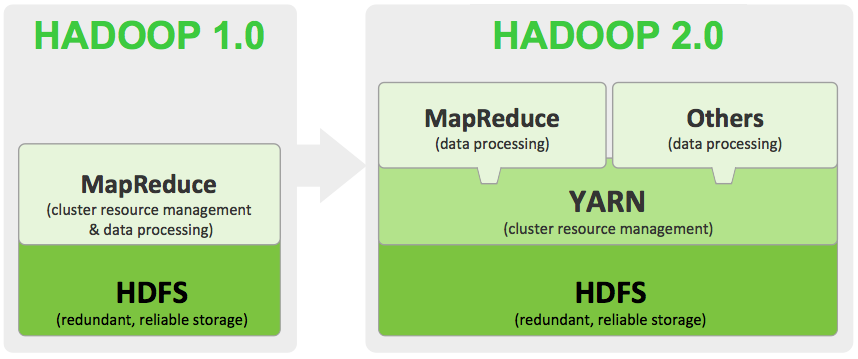
\includegraphics[width=\linewidth]{hadoop1vshadoop2}
		\caption[Differences entre Hadoop 1.0 et Hadoop 2.0]{Differences entre Hadoop 1.0 et Hadoop 2.0\footnotemark}
	\end{figure}

	\footnotetext{\url{https://infinitescript.com/wordpress/wp-content/uploads/2014/08/Differences-between-Hadoop-1-and-2.png}}

A ce jour, Hadoop est à la version 3.3.0.
Dans sa version 1 (Figure 2 - 1, Hadoop 1.0) les composants de base d’Hadoop sont: le modèle MapReduce qui est responsable du traitement distribué et la gestion des ressources du cluster, et HDFS (Hadoop Distributed File system) pour la réalisation du stockage distribué.
Dans sa version 2 (Figure 2 - 1, Hadoop 2.0) le modèle MapReduce joue seulement le rôle de traitement distribué et Yarn est devenue le gestionnaire de ressources du cluster.
Cela permet à Hadoop d'avoir autour de lui tout un écosystème incluant d’autres Frameworks capables de faire des traitements de données distribués tout en ajoutant des nouvelles structures et des nouvelles façons de faire fonctionner Hadoop au niveau applicatif qu’au niveau d’exécution.
Enfin la version 3 introduit des ameliorations visant de reduire le cout de stockage néccesaire pour assurer la tolerance aux pannes et d'optimiser la gestion des ressources pour assurer une scalabilité encore supériore.

Dans les sections suivantes de ce chapitre, on verra plus en détails le fonctionnement de MapReduce, d’HDFS, Yarn, l’écosystème autour d’Hadoop, une mise en œuvre d’Hadoop avec un exemple d’exécution de MapReduce, et enfin Apache Hive et Apache Spark et comment les implémenter avec des exemples.

	\section{MapReduce}
MapReduce est un paradigme visant à simplifier le traitement de données sur de grands clusters tout en assurant la fiabilite du traitement et la tolerance aux pannes.
Son principe se base sur la technique "diviser pour régner" - il decoupe le traitement en sous-traitements et les execute en parallele sur le cluster.

Dans un processus MapReduce 4 étapes peuvent être distinguées.
Le programme exécuté reçoit à l’entrée (Input) un groupement de donnée provenant de HDFS, procède aux 4 étapes (Découper, Mapper, Grouper, Réduire) et le résultat final en sortie sera mise dans HDFS.

\paragraph{Les 4 étapes réalisées lors d’un MapReduce :}

\begin{itemize}  
\item 
Découper (Split) : Rendre les données en entrée en plusieurs fragments pour former des sous-ensembles de données selon une indice telle qu'une espace, une virgule, point-virgule, une nouvelle ligne ou une autre regle logique.
\item
Map : Convertir chacun des fragments en un autre sous ensemble de données où les éléments forment des couples (clef ; valeur).   
\item
Grouper (Shuffle) : Unir l’ensemble des couples (clef ; valeur) issue de la totalité des taches Map par clef.  
\item
Réduire (Reduce) : Combiner l’ensembles des couples indexés par clef en formant des groupements ayant chacun une clef distinctes associé à sa valeur.  C’est une agrégation en un sous ensemble de données formant des couples (clef ; valeur) ayant pour clef l’identifiant de l’enregistrement, et valeur, la valeur de l’enregistrement.
\end{itemize}


\paragraph{La forme générale d’un MapReduce est de la sorte :}\mbox{}\\

Map		(k1, v1)		->		list(k2, v2)

Reduce	(k2, list(v2))	->		list(v2)

\paragraph{Regardons un peu plus près dans un exemple d’application MapReduce, Compteur de mots la réalisation de ces processus (voir Figure 2 - 2).}

\newpage

\begin{figure}[ht]
	\centering
	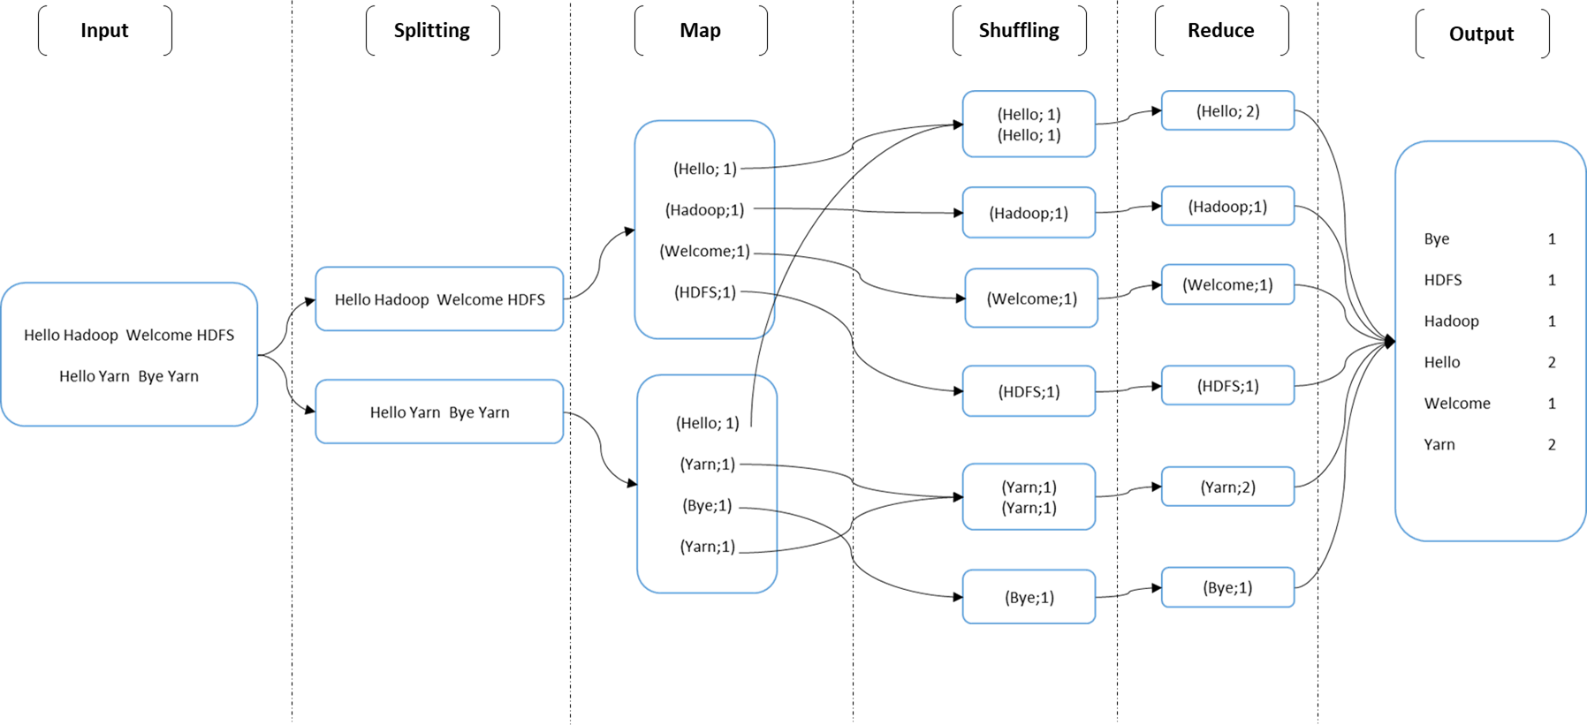
\includegraphics[width=\linewidth]{mapReduceSchema}
	\caption{Schéma des étapes du paradigme MapReduce illustré de l’exemple compteur de mots}
\end{figure}

Dans le tableau suivant (Tableau 2 - 1), on verra pour les différentes fonctions Map et Reduce la forme des données en entrée et en sortie pour chacune d’elles.

\begin{table}[H]
	\begin{tabular}{|p{1.4cm}|p{3.4cm}|p{1.5cm}|p{3.3cm}|p{2cm}|}
		\hline
		\rowcolor[HTML]{CBCEFB} 
		Fonction & Entrée/Input & Type de valeur d’entrée & Sortie/Output & Type de valeur de sortie \\
		\hline
		Map & 
		Hello Hadoop Welcome HDFS Hello Yarn Bye Yarn &
		Un ensemble de données &
		(Hello;1), (Hadoop;1), (Welcome;1), (HDFS;1), (Hello; 1), (Yarn;1), (Bye;1), (Yarn;1) &
		Un ensemble de données en (Clef ; valeur) \\
		\hline
		Reduce & 
		(Hello; 1), (Hadoop;1), (Welcome;1), (HDFS;1), (Hello; 1), (Yarn;1), (Bye;1), (Yarn;1) & 
		Un ensemble de couples (Clef ; valeur) & 
		(Bye; 1), (HDFS; 1), (Hadoop; 1), (Hello; 2), (Welcome; 1), (Yarn; 2) &
		Un sous-ensemble de couples (Clef ; valeur) \\
		\hline
	\end{tabular}
	\caption{Exemple MapReduce}
\end{table}
  
\section{HDFS}

HDFS (Hadoop Distributed File system) est le système de fichier distribué d’Hadoop.
Ce système de fichier peut être comparé à d’autres systèmes de fichiers tel que Ext, Ext2, Ext3, Ext4, FAT32, NTFS, HFS+ et autres.
La différence entre ces systèmes de fichiers est que celui d’Hadoop est distribué.

HDFS a le même concept de stockage en bloc.
Dans les systèmes de fichier il est environ de quelques Kilo-octets (normalement 512 Ko) tandis qu’un bloc dans HDFS est par défaut de 128 Mo (modifiable dans la configuration).
A ne pas confondre un bloc dans le disque et un bloc dans HDFS.
Un fichier de 1 Mo stocké dans HDFS à un bloc de taille 128 Mo mais utilise 1 Mo de disque physique.
La raison est de minimiser le coût de recherches des blocks dans le disque.
Tant la vitesse des disques augments, tant, la tendance est d’augmenter la taille de block dans HDFS. 
Hadoop est dit un système de fichier distribué, les blocs de données sont repartis sur toutes les machines du cluster et donne une vision d’une seule machine à disque unique.
Car il permet dans un seul point d’avoir accès aux données reparties sur l’ensemble du cluster.
Les blocs de données sont aussi répliqués de telle sorte que si une machine tombe en panne sur le cluster, le système continuera à être disponible et de fonctionner sans perturbation, ni perte de données.

Hadoop supporte 3 modes d’installation: « Local (Standalone) », « Pseudo-Distributed », « Fully- Distributed ». Par défaut, Hadoop est configure en mode “Standalone” qui fonctionne dans un mode non-distribué dans un seul processus Java.  Dans une configuration « Pseudo-Distributed » tous les démons d’Hadoop sont exécutés dans des processus Java distincts sur un seul nœud (machine). Une configuration « Fully- Distributed » fonction sur plusieurs machines formant un cluster où chaque machine exécute séparément leur démon respectif.

\newpage
\begin{figure}[t]
	\centering
	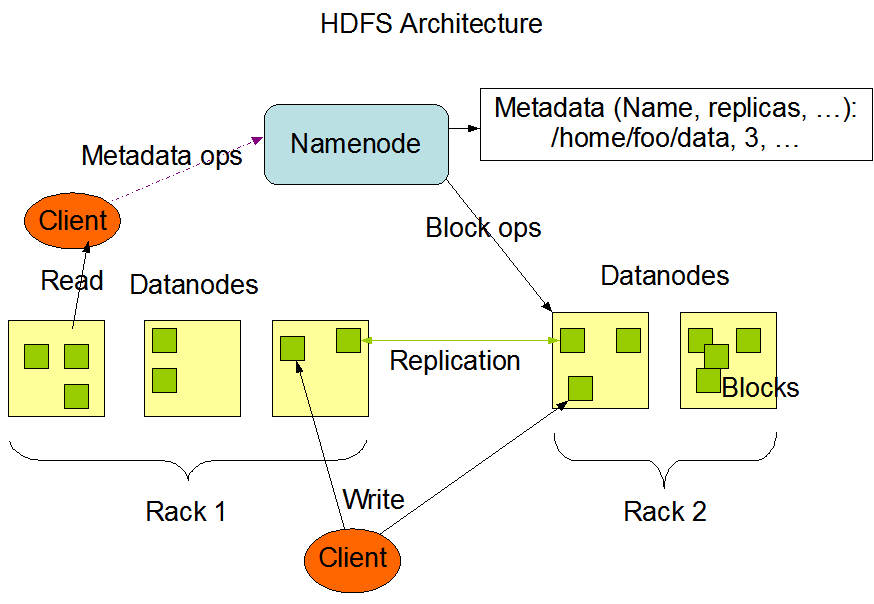
\includegraphics[width=\linewidth]{hdfsArch}
	\caption[Schéma de l'architecture du mode fonctionnement d'HDFS ]{Schéma de l'architecture du mode fonctionnement d'HDFS \footnotemark}
\end{figure}
\footnotetext{Source : \url{https://hadoop.apache.org/docs/r1.2.1/hdfs\_design.html}}

\paragraph{Le fonctionnement d’HDFS (Figure 2 - 3) se base sur 2 démons, NameNode et DataNode :}

\begin{itemize}
	\item
	Le NameNode, démon du nœud maitre, le seul pour tout le cluster, stocke les métadonnées concernant le nom, son répertoire, le positionnement des blocks et des réplicas sur le cluster.
	\item
	Le DataNode s’exécutant sur les autres machines du cluster participe au stockage des blocs d’information sur leurs disques.  Il est en perpétuel contact avec le NameNode pour tout échange (demande de stockage de blocs, les informations sur les blocs contenue, les statuts, etc.).   Les DataNodes communiquent entre eux pour effectuer la réplication des données et signalent le NameNode de son contenue actuel.
\end{itemize}
\paragraph{}
Un client qui veut lire ou écrire un fichier dans HDFS contacte le NameNode pour savoir ou récupérer ou stocker les blocs de ce dernier.

HDFS est utilisé non seulement pour le stockage des données usuelles, mais aussi le stockage de données temporaires issue des étapes intermédiaires des applications lors de leurs exécutions, et les résultats finals de l’exécution des applications.     

\section{Yarn}

Yarn est le gestionnaire de ressource d’Hadoop qui effectue la distribution des taches sur l’ensemble des machines du cluster Hadoop et fait le suivie de l’état des taches en exécution. 

\begin{figure}[ht]
	\centering
	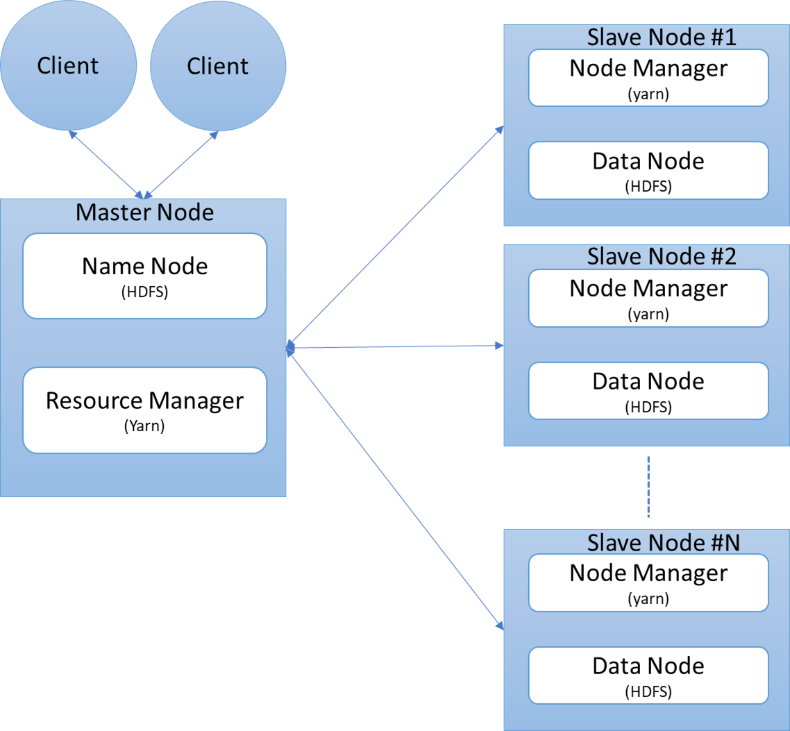
\includegraphics[width=10cm]{demonsSchema}
	\caption{Schéma de positionnement des différents démons sur le cluster}
\end{figure}

Dans l’architecture d’Hadoop Yarn dans un cluster (Figure 2 - 4), le NameNode (nœud Maitre) comporte le ResourceManager et les DataNode (nœud Esclave) comportent chacun un NodeManager.

Comme montre, les deémons de HDFS sont

Comme on peut le voir dans le schéma suivant (Figure 2 - 5) le role de chaque elements au niveau du cluster lorsqu’un ou plusieurs clients envoient une application à être executée.

\begin{figure}[ht]
	\centering
	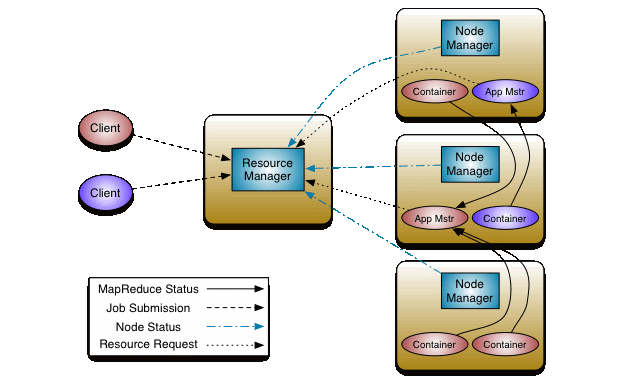
\includegraphics[width=10cm]{yarnArch}
	\caption[Schéma de l'architecture de fonctionnement de Yarn]{Schéma de l'architecture de fonctionnement de Yarn \footnotemark}
\end{figure}

\footnotetext{Source : \url{https://hadoop.apache.org/docs/stable/hadoop-yarn/hadoop-yarn-site/YARN.html}}

Un \textbf{Client} peut envoyer n’importe quel type d’application reconnue par Yarn. 

Le \textbf{ResourceManager} fait le suivie des NodeManagers et des ressources disponibles.
Il gère l’allocation des ressources disponibles aux applications et aux taches en évaluant le ou les nœuds les plus optimisés à recevoir l’ensemble des processus à exécuter.
En prenant en compte la demande du client, le ResourceManager demande au NodeManager de recevoir une applicationMaster et crée un Container pour son exécution.

Le \textbf{NodeManager} fournit pour sa part des ressources pour effectuer les calculs sous forme de conteneurs (Containers) et fait la gestion des processus exécutés par les conteneurs.

L’\textbf{ApplicationMaster} fait la coordination de toutes ses taches en exécution c’est-à-dire les taches qui ont rapport à sa propre application.
Elle fait la demande pour avoir des conteneurs adéquate pour l’exécution de ses taches.

Les \textbf{Containers} (Conteneurs) sont des ressources capables d’exécuter différents types de taches (Application Masters, Map, Reduce, …) et peut être dimensionner selon les besoins en termes de RAM et de CPU.

\section{Ecosystème Hadoop}

Hadoop est un Framework qui comprend une panoplie d’outils et technologies autour de lui. Ainsi nous parlons de l’écosystème d’Hadoop. Avant de commencer à travailler avec Hadoop, il est tant essentiel de comprendre son environnement. Chaque outil peut jouer un rôle concret dans différentes parties d’un Project Big Data. La connaissant de son environnement permet de choisir les technologies adéquates pour une meilleur organisation, optimisation de son projet.

L’écosystème d’Hadoop (décrit dans Figure 2- 6) est composé de ces composants principaux (HDSF, MapReduce, Yarn invoquer dans les sections précédentes) et un ensemble d’outils, pour la majorité des projets open-sources d’Apache Software Fondation et des solutions propriétaires.  Tous les outils dans son écosystème ont pour but principale l’ingestion, le stockage, l’analyse de données et la maintenance du système. 

\begin{figure}[ht]
	\centering
	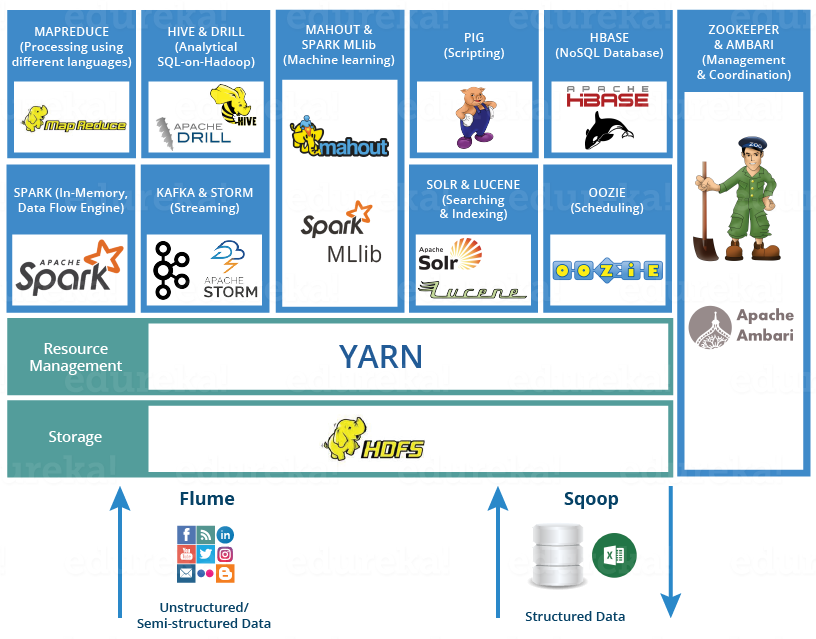
\includegraphics[width=10cm]{hadoopEco}
	\caption[Schéma de représentation de l'écosystème d'Hadoop]{Schéma de représentation de l'écosystème d'Hadoop \footnotemark}
\end{figure}

\footnotetext{Source : \url{https://cdn.edureka.co/blog/wp-content/uploads/2016/10/HADOOP-ECOSYSTEM-Edureka.png}}

Le nombre d’outils autour d’Hadoop ne cesse d’augmenter. Dans cette section, on verra un aperçu des outils les plus utilisés actuellement sur le marché dans le domaine du Big Data.


\subsection{Hive}

Apache Hive \footnote{Voir https://hive.apache.org/} est un Framework de Data Warehousing permettant à partir d’un interface SQL-like d’effectuer lecture, écriture et   la gestion de grand volume de données dans un environnement distribué.

\subsection{Spark}

Apache Spark \footnote{Voir https://spark.apache.org/} est un Framework pour procéder à de l’analyse de données en utilisant des processus de traitement de données en mémoire dans un environnement distribué.

\subsection{Sqoop}

Apache Sqoop \footnote{Voir http://sqoop.apache.org/} est un outil de type ETL (Extract, Transform, Load) conçu pour effectuer des transferts de données en boucle entre Hadoop et les données structurée (base de données relationnelle, fichier CSV, …) sur de gros volume de manière efficacement.  

\subsection{Hbase}

Apache HBase \footnote{Voir https://hbase.apache.org/} est une base de données Hadoop ayant la capacité de gérer l’accès en lecture et écriture de grand volume de données de façon aléatoire et en temps réel. HBase est une base capable de maintenir de très grandes tables pouvant contenir des millions de colonnes.    

\subsection{Pig}

Apache Pig \footnote{Voir https://pig.apache.org/} est une plateforme pour effectuer l’analyse de données sur de grand volume de données. Son langage de très haut niveau, Pig Latin, un langage très textuel ayant des structures de commandes semblable à SQL. Lors de sa compilation, il produit de séquences de tâches Map et Reduce déjà capable d’être parallélisé sur Hadoop.  

\subsection{Zookeeper}

Apache Zookeeper \footnote{Voir https://zookeeper.apache.org/} est un gestionnaire de service centralisé dans un environnement distribué. Il permet dans un seul endroit de faire maintenance les informations de configuration et fournit la synchronisation d’information distribué et des services d’énumération et de regroupement.   

\subsection{Ambari}

Apache Ambri \footnote{Voir https://ambari.apache.org/} est un outil de gestion qui offre des services simplifiant l’approvisionnement de nouveau service et de sa configuration, la gestion et la surveillance dans des clusters d’Hadoop.

\subsection{Oozie}

Apache Oozie \footnote{Voir http://oozie.apache.org/} est système de planification et de déclenchement d’événement dans Hadoop. Il peut être considéré comme un service d’horloge ou d’alarme interne à Hadoop. Il a la capacité d’exécuter un ensemble d’évènements une après l’autre ou de déclencher des évènements par rapport à la disponibilité d’information. Les évènements lancés peuvent être des taches map-reduce, Pig, Hive, Sqoop ou programme Java, etc. 

\subsection{Apache Solr et Lucene}

Apache Solr et Apache Lucene \footnote{Voir http://lucene.apache.org/solr/} sont une combinaison de deux (2) services qui sont utilisés pour la recherche et l’indexation dans l’environnement Hadoop.  Il est adapté pour la réalisation de système d’information nécessitant la recherche sur des textes intégral. Lucene est un composant cœur et Solr est bati autour de lui ajoutant encore plus de fonctionnalité.  

\subsection{Kafka}

Apache Kalka est un système de messagerie distribué permettant la publication, l’abonnement et l’enregistrement des échanges de flux de données. Il permet la création d’un pipeline de diffusion de données entre des systèmes ou des applications. 

\subsection{Storm}

Apache Storm est un système de traitement d’informations diffusées en temps réel d’Hadoop pour la réalisation de cas d’usage d’analyse en temps réel, du Machine Learning, la surveillance d’opérations en continue.

\subsection{Flume}

Apache Flume est un service distribué de collecte, d’agrégation, de transfert de grand volume de données semi-structurées ou non-structurées de flux en ligne dans HDFS. Ces données sont en provenance de serveur web tel que les fichiers journaux, le trafic réseau, les médias sociales, etc.

\subsection{Drill}

Apache Drill est moteur de requête SQL sans schéma pour Hadoop, NoSQL, et Cloud Storage. Il supporte une variété de base de données NoSQL et est capable d’effectuer des requêtes de jointure entre multi-sources de données.  

\subsection{Mahout}

Apache Mahout \footnote{Voir http://mahout.apache.org/} fournit un environnement pour le développement d’application de Machine Learning à des performances scalable.

\subsection{Impala}

Apache Impala \footnote{Voir https://impala.apache.org/} (en projet d’incubation chez Apache) et Presto \footnote{Voir https://prestodb.io/} donnent une bonne appréciation très prometteuse d’eux même dès leur début.
Tous les deux sont des moteurs de requête SQL pour les données du Big data. Ils sont capables très rapidement de traiter des données sur des Pétaoctets. Des chercheurs ont publié, chez Cloudera en 2015 « Impala : A Modern, Open-Source SQL Engine for Hadoop » \footnote{M. Kornacker et al., « Impala: A Modern, Open-Source SQL Engine for Hadoop. », in CIDR, 2015, vol. 1, p. 9.} et chez Facebook en 2013 « Presto : Interacting with petabytes of data at Facebook » \footnote{“Presto: Interacting with petabytes of data at Facebook.” [En Ligne]. Disponible : https://www.facebook.com/notes/facebookengineering/presto-interacting-with-petabytes-of-data-atfacebook/10151786197628920.}

\section{Installation de Hadoop 2.8.0 en cluster sur Linux Ubuntu 16.04.1 TLS}

Cette section montre la configuration de Apache Hadoop dans sa version 2.8.0 en cluster avec Yarn comme gestionnaire de ressources. Comme on peut voir sur le schéma suivant (Figure 2 - 7 ), l’installation se fera sur trois (3) machine avec un Nœud Maitre (Master) et  deux (2) Nœuds Esclaves (Slave1 et Slave2). 


\begin{figure}[ht]
	\centering
	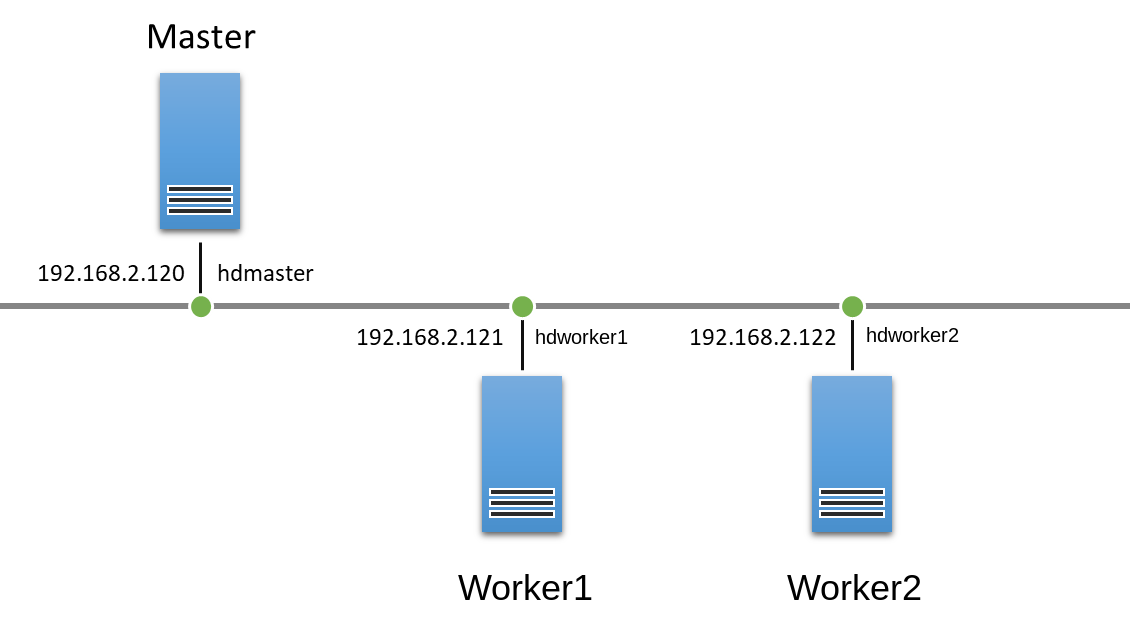
\includegraphics[width=\linewidth]{clusterSchema}
	\caption{Schéma de configuration du cluster d'Hadoop}
\end{figure}

Cette Installation sera effectuée sur 3 Machine virtuelle sur VirtualBox avec une capacité de 4Go de RAM, de 20Go de disque et de 4 Cœurs alloués chacune. Avec un processus définit comme tel : « Intel(R) Core(TM) i7-6700HQ CPU @ 2.60GHz, 2601 Mhz, 4 Core(s), 8 Logical Processor(s) ». Le système d’exploitation utilisé sera la version de Ubuntu 16.04.1 TLS.

\subsection{Prérequis}

Dans cette section, nous verrons les configurations préliminaires pour le fonctionnent d’Apache Hadoop et quelques bonnes pratiques.
Hadoop étant une plateforme basée sur Java, pour qu’elle puisse fonctionner, il a besoin de la machine virtuel Java (JVM) pour s’exécuter.
Hadoop peut fonctionner sur les toutes les versions de java supérieure à la version 1.5.
Un autre aspect important est que Hadoop utilise « SSH » pour la connexion entre les différents nœuds de l’écosystème distribué.
Hadoop fait usage de SSH pour accéder en aux nœuds esclaves pour démarrer et faire la gestion services HDFS et MapReduce de son environnement.
Et pour éviter des problèmes de sécurité, une mise en place d’utilisateur dédié est nécessaire pour l’exécution de toutes les activités en rapport avec Hadoop.
Ce qui permettra au divers nœud de communiquer entre eux sans utilisation de mot de passe à partir des clés RSA générées. 
Ces prérequis doivent être réalisés sur toutes les machines qui feront partie du cluster Hadoop.

\subsubsection{Installation d’Oracle Java version 8}

Dans le terminal:

\begin{lstlisting}[language=bash, frame=single]
sudo add-apt-repository ppa:webupd8team/java
\end{lstlisting}

Mise à jour de la base de référence des packages sur la machine :

\begin{lstlisting}[language=bash, frame=single]
sudo apt-get update
\end{lstlisting}

Installation de java 8 :

\begin{lstlisting}[language=bash, frame=single]
sudo apt-get install oracle-java8-installer
\end{lstlisting}

Faire d’Oracle java 8 par comme version par défaut :

\begin{lstlisting}[language=bash, frame=single]
sudo apt-get install oracle-java8-set-default
\end{lstlisting}

Vérifier si tout est correct :

\begin{lstlisting}[language=bash, frame=single]
java -version
\end{lstlisting}

Informations qui devrait voir afficher :  
\begin{lstlisting}[language=bash, frame=single]
java version "1.8.0_131"
Java(TM) SE Runtime Environment (build 1.8.0_131-b11)
Java HotSpot(TM) 64-Bit Server VM (build 25.131-b11,
mixed mode)
\end{lstlisting}

\subsubsection{Configuration du Hostname}

Dès le début, il faut déterminer les noms des « hostname » et les adresses IP associées à chaque machine.  Notre nœud maitre, Master node est hdmaster et nos nœuds esclaves, « Slave node », sont respectivement hdslave1 et hdslave2. Assurer que chaque nœud ait une adresse IP « static » pour qu’elle ne change pas au démarrage ou autre. Cela peut se faire à partir du fichier de configuration réseau (/etc/network/interfaces)

\begin{lstlisting}[language=bash, frame=single]
sudo nano /etc/hosts
\end{lstlisting}

Ajoute dans le fichier \textbf{/etc/hosts} les lignes suivantes avec l’\textbf{adresse IP, un alias et le hostname} correspondant à chaque nœud

\begin{lstlisting}[language=bash, frame=single]
# ip and hostname for hadoop configuration
192.168.2.120  hdmaster hdpdb-master
192.168.2.121  hdslave1  hdpdb-slave1
192.168.2.122  hdslave2  hdpdb-slave2
\end{lstlisting}

\subsubsection{Création d’un utilisateur Hadoop pour l’accès HDFS et MapReduce}

Nous allons procéder à la création hadoop en tant que groupe système et hdb en tant que compte utilisateur garant du système Hadoop

\begin{lstlisting}[language=bash, frame=single]
sudo adduser -ingroup hadoop hdp
\end{lstlisting}

Tous les nœuds du cluster Hadoop doit avoir le même nom d’utilisateurs pour exécuter ses activités.

\subsubsection{Installation de SSH}

\begin{lstlisting}[language=bash, frame=single]
sudo apt-get install ssh
\end{lstlisting}

Configuration de SSH pour l’utilisateur Hadoop hdb


\begin{lstlisting}[language=bash, frame=single]
sudo su hdb
ssh-keygen -t rsa -P " "
cat $HOME/.ssh/id_rsa.pub >> $HOME/.ssh/authorized_keys
\end{lstlisting}

Copier les clés SSH depuis Master vers Slaves pour initier un accès SSH sans mot de passe 

\begin{lstlisting}[language=bash, frame=single]
ssh-copy-id -i $HOME/.ssh/id_rsa.pub hdb@hdslave2
ssh-copy-id -i $HOME/.ssh/id_rsa.pub hdd@hdslave2
\end{lstlisting}

\subsection{Installation d'Hadoop}

Téléchargement de Hadoop (ici on fera usage de la version 2.8.0).

La version binaire d’Apache Hadoop peut être récupéré sur le site officiel (http://www.hadoop.apache.org).

Allez dans le répertoire partager pour que Hadoop puisse être exécuté par un utilisateur autre.  Nous faisons le choix du répertoire /usr/local/ pour l’installation.


\begin{lstlisting}[language=bash, frame=single]
cd /usr/local/
\end{lstlisting}

Téléchargement du fichier archive d’Hadoop

\begin{lstlisting}[language=bash, frame=single]
sudo wget 
http://mirror.ibcp.fr/pub/apache/hadoop/common/hadoop-
2.8.0/hadoop-2.8.0.tar.gz
\end{lstlisting}

Désarchiver le fichier nouvellement téléchargé (ici Hadoop-2.8.0.tar.gz)

\begin{lstlisting}[language=bash, frame=single]
sudo tar xzf hadoop-2.8.0.tar.gz
\end{lstlisting}

Donner l’utilisateur hdb la propriété sur le répertoire

\begin{lstlisting}[language=bash, frame=single]
sudo chown hdb:hadoop -R /usr/local/hadoop-2.8.0
\end{lstlisting}

\paragraph{Mise en place des variables d’environnement d’Hadoop}\mbox{}\\


Se connecter en tant que hdb

\begin{lstlisting}[language=bash, frame=single]
sudo su hdp
\end{lstlisting}

Ajouter les variables d’environnement d’Hadoop dans le fichier profile de l’utilisateur hdb

\begin{lstlisting}[language=bash, frame=single]
nano /home/hdb/.bashrc
\end{lstlisting}

\begin{lstlisting}[language=bash, frame=single]
#Add to the end of this file 
## BEGIN -- HADOOP ENVIRONMENT VARIABLES
export JAVA_HOME=/usr/lib/jvm/java-8-oracle
export HADOOP_HOME=/usr/local/hadoop-2.8.0
export PATH=$PATH:$HADOOP_HOME/bin
export PATH=$PATH:$HADOOP_HOME/sbin
export HADOOP_MAPRED_HOME=$HADOOP_HOME
export HADOOP_COMMON_HOME=$HADOOP_HOME
export HADOOP_HDFS_HOME=$HADOOP_HOME
export YARN_HOME=$HADOOP_HOME
export HADOOP_COMMON_LIB_NATIVE_DIR=$HADOOP_HOME/lib/native
export HADOOP_OPTS="-Djava.library.path=$HADOOP_HOME/lib"
## END-- HADOOP ENVIRONMENT VARIABLES
\end{lstlisting}

Rendre la modification du fichier profile active immédiatement

\begin{lstlisting}[language=bash, frame=single]
source /home/hdb/.bashrc
\end{lstlisting}

Modifier le fichier de configuration de l’environnement d’Hadoop 

\begin{lstlisting}[language=bash, frame=single]
nano / usr/local/hadoop-2.8.0/etc/hadoop/hadoop-env.sh
\end{lstlisting}

\begin{lstlisting}[language=bash, frame=single]
##modifier la ligne 
JAVA_HOME=/usr/lib/jvm/java-8-oracle
\end{lstlisting}

Tester si Hadoop fonctionne

\begin{lstlisting}[language=bash, frame=single]
hadoop version
\end{lstlisting}

A ce niveau, Hadoop est dans sa configuration par défaut, ce qui veut dire aussi qui se trouve en mode « stand Alone ».

\subsection{Configuration de Hadoop en mode « Full Distributed Cluster »}

\subsubsection{Création des répertoires de données temporaires d’Hadoop}

Dans le nœud maitre :

\begin{lstlisting}[language=bash, frame=single]
sudo mkdir -p /usr/local/tmp_hadoop/

sudo mkdir -p /usr/local/tmp_hadoop/hdfs/namenode

sudo chown hdb:hadoop -R  /usr/local/tmp_hadoop/
\end{lstlisting}

Dans les nœuds esclaves :

\begin{lstlisting}[language=bash, frame=single]
sudo mkdir -p /usr/local/tmp_hadoop/

sudo mkdir -p /usr/local/tmp_hadoop/hdfs/datanode

sudo chown hdb:hadoop -R  /usr/local/tmp_hadoop/
\end{lstlisting}

\subsubsection{Editer le fichier « masters »}

Dans le nœud maitre

\begin{lstlisting}[language=bash, frame=single]
nano /usr/local/hadoop-2.8.0/etc/hadoop/masters 
\end{lstlisting}


\begin{lstlisting}[language=bash, frame=single]
## Add name of master nodes

hdmaster
\end{lstlisting}

\subsubsection{Editer le fichier « slaves »}

Dans le nœud maitre


\begin{lstlisting}[language=bash, frame=single]
nano /usr/local/hadoop-2.8.0/etc/hadoop/slaves 
\end{lstlisting}

\begin{lstlisting}[language=bash, frame=single]
## add all slaves hostname or IP address
hdslave1
hdslave2
\end{lstlisting}

\subsubsection{Editer le fichier « core-site.xml »}

Dans le nœud maitre et les nœuds esclaves :


\begin{lstlisting}[language=bash, frame=single]
nano /usr/local/hadoop-2.8.0/etc/hadoop/core-site.xml
\end{lstlisting}

\begin{lstlisting}[language=bash, frame=single]

<configuration>
<property>
<name>fs.default.name</name>
<value>hdfs://hdmaster:9000</value>
</property>
</configuration>

\end{lstlisting}

\subsubsection{Editer le fichier « hdfs-site.xml »}

Dans le nœud maitre

\begin{lstlisting}[language=bash, frame=single]
nano /usr/local/hadoop-2.8.0/etc/hadoop/hdfs-site.xml 
\end{lstlisting}

\begin{lstlisting}[language=bash, frame=single]
<configuration>
<property>
      <name>dfs.replication</name>
      <value>3</value>
 </property>
 <property>
      <name>dfs.permissions</name>
      <value>false</value>
 </property>
<property>
<name>dfs.namenode.name.dir</name>
<value>/usr/local/tmp_hadoop/hdfs/namenode</value>
</property>
</configuration>
\end{lstlisting}

Dans les nœuds esclaves :

\begin{lstlisting}[language=bash, frame=single]
<configuration>
<property>
      <name>dfs.replication</name>
      <value>3</value>
 </property>
 <property>
      <name>dfs.datanode.data.dir</name>
      <value>/usr/local/tmp_hadoop/hdfs/datanode</value>
 </property>
</configuration> 
\end{lstlisting}

\subsubsection{Editer le fichier « yarn-site.xml »}

Dans le nœud maitre et les nœuds esclaves


\begin{lstlisting}[language=bash, frame=single]
nano /usr/local/hadoop-2.8.0/etc/hadoop/yarn-site.xml 
\end{lstlisting}

\begin{lstlisting}[language=bash, frame=single]

<configuration>
<property>
      <name>yarn.resourcemanager.hostname</name>
      <value>hdmaster</value>
</property>
<property>
      <name>yarn.resourcemanager.address</name>
      <value>hdmaster:8032</value>
</property>
<property>
      <name>yarn.resourcemanager.scheduler.address</name>
      <value>hdmaster:8030</value>
</property>
<property>
      <name>yarn.resourcemanager.resource-tracker.address</name>
      <value>hdmaster:8031</value>
</property>
<property>
      <name>yarn.nodemanager.aux-services</name>
      <value>mapreduce_shuffle</value>
</property>
<property>
      <name>yarn.nodemanager.aux-services.mapreduce.shuffle.class</name>
      <value>org.apache.hadoop.mapred.ShuffleHandler</value>
</property>
</configuration>
\end{lstlisting}

\subsubsection{Editer le fichier « mapred-site.xml »}

Dans le nœud maitre et les nœuds esclaves

\begin{lstlisting}[language=bash, frame=single]
cp   /usr/local/hadoop-2.8.0/etc/hadoop/mapred-site.xml.template   /usr/local/hadoop-2.8.0/etc/hadoop/mapred-site.xml

nano /usr/local/hadoop-2.8.0/etc/hadoop/mapred-site.xml
\end{lstlisting}

\begin{lstlisting}[language=bash, frame=single]
<configuration>
<property>
      <name>mapreduce.framework.name</name>
      <value>yarn</value>
</property>
<property>
        <name>mapreduce.job.tracker</name>
        <value>hdmaster:9001</value>
</property>
</configuration>
\end{lstlisting}

\subsubsection{Formattage du Namenode}

Dans le nœud maitre, pour une première utilisation, il faut formater le Namenode à partir d’HDFS.


\begin{lstlisting}[language=bash, frame=single]
hdfs namenode -format
\end{lstlisting}

\subsection{Démarrage des services des démons d’Hadoop sur le cluster}

\subsubsection{Lancement du daemon hdfs}

Dans le nœud maitre :
Passer cette commande pour démarrer le démon HDFS

\begin{lstlisting}[language=bash, frame=single]
start-dfs.sh
\end{lstlisting}

Passer cette commande pour vérifier qu’ils sont bien démarrés 

\begin{lstlisting}[language=bash, frame=single]
jps
\end{lstlisting}

\begin{lstlisting}[language=bash, frame=single]
8561 Jps
7604 NameNode
7964 SecondaryNameNode
\end{lstlisting}

Voici ce que vous devez voir 

Dans les nœuds esclaves :

En lançant depuis le nœud maitre le démon, il activera ceux des nœuds esclaves à travers SSH. Aucune action est nécessaire sur les nœuds esclaves. 

Passer cette commande pour vérifier qu’ils sont bien démarrés 

\begin{lstlisting}[language=bash, frame=single]
jps
\end{lstlisting}

\begin{lstlisting}[language=bash, frame=single]
8561 Jps
7753 DataNode
\end{lstlisting}

\subsubsection{Lancement du daemon de Yarn}

Dans le nœud maitre:
Passer cette commande pour démarrer Yarn

\begin{lstlisting}[language=bash, frame=single]
start-yarn.sh
\end{lstlisting}

Passer cette commande pour vérifier qu’ils sont bien démarrés 

\begin{lstlisting}[language=bash, frame=single]
jps
\end{lstlisting}

\begin{lstlisting}[language=bash, frame=single]
8128 ResourceManager
8561 Jps
7604 NameNode
7964 SecondaryNameNode
\end{lstlisting}

Voici ce que vous devez voir 

Dans les nœuds esclaves : 

Pour les mêmes raisons dites tantôt, aucune action est nécessaire sur les nœuds esclaves.

Passer cette commande pour vérifier qu’ils sont bien démarrés 

\begin{lstlisting}[language=bash, frame=single]
jps
\end{lstlisting}

\begin{lstlisting}[language=bash, frame=single]
8561 Jps
8249 NodeManager
7753 DataNode
\end{lstlisting}

Voici ce que vous devez voir 

Pour l’arrêter les démons d’Hadoop, lancer successivement le fichier \textbf{stop-dfs.sh} et \textbf{stop-yarn.sh} en étant l’utilisateur propriétaire d’Hadoop. Dans notre cas, l’utilisateur est \textbf{hdb}.

\paragraph{Configuration de Yarn et MapReduce pour la gestion et optimisation des ressources}\mbox{}\\

Yarn et MapReduce viennent avec une configuration par défaut. 
En ajoutant des paramètres dans les fichiers « mapred-site.xml », « yarn-site.xml » et « capacity-scheduler.xml » signifient pour Hadoop qu’il doit considérer ces nouvelles propriétés inscrites au lieu des valeurs par défaut.
Dans le but de la gestion et de l’optimisation des ressources partagé et d’utilisation de la mémoire, il faut savoir ou regarder pour trouver l’équilibre idéale pour le bon fonctionnement du système.
Une configuration peut bien marché pour une application et non pour une autre par rapport au volume de mémoire demandé au ressources disponible.
Anisi, fréquemment des processus d'exécution de plusieurs applications échoue car la taille de mémoire d'ApplicationMaster et d'autres conteneurs dépassent largement la capacité disponible.
Ce qui peut impliquer une acceptation de l’application pour être exécuter et que le processus soit resté en fil d’attente ou un arrêt brutal du processus au cours de son exécution.

Les tableaux suivants décrivent la valeur par défaut et la valeur actuelle des propriétés d’ajustement dans leur fichier respectif. 

\paragraph{mapred-site.xml}\mbox{}\\

\begin{table}[H]
\begin{tabular}{llll}
\rowcolor[HTML]{4472C4} 
{\color[HTML]{FFFFFF} Nom du propriété} & {\color[HTML]{FFFFFF} Valeur par défaut} & {\color[HTML]{FFFFFF} Valeur actuelle} & {\color[HTML]{FFFFFF} description} \\
\rowcolor[HTML]{D9E2F3} 
mapreduce.map.memory.mb                 & 1204                                     & 256                                    &                                    \\
mapreduce.reduce.memory.mb              & 3072                                     & 256                                    &                                    \\
\rowcolor[HTML]{D9E2F3} 
mapreduce.map.java.opts                 & -Xm900m                                  & -Xmx205m                               &                                    \\
mapreduce.reduce.java.opts              & -Xm2560m                                 & -Xmx205m                               &                                    \\
\rowcolor[HTML]{D9E2F3} 
yarn.app.mapreduce.am.resource.mb       & 1536                                     & 768                                    &                                    \\
yarn.app.mapreduce.am.command-opts      & -Xm1024m                                 & -Xmx615m                               &                                   
\end{tabular}
\caption{}
\end{table}

\paragraph{yarn-stie.xml}\mbox{}\\

\begin{table}[H]
\begin{tabular}{llll}
\rowcolor[HTML]{4472C4} 
{\color[HTML]{FFFFFF} Nom du propriété}  & {\color[HTML]{FFFFFF} Valeur par défaut} & {\color[HTML]{FFFFFF} Valeur actuelle} & {\color[HTML]{FFFFFF} description} \\
\rowcolor[HTML]{D9E2F3} 
yarn.nodemanager.resource.memory-mb      &                                          & 2048                                   &                                    \\
yarn.scheduler.minimum-allocation-mb     & 1024                                     & 256                                    &                                    \\
\rowcolor[HTML]{D9E2F3} 
yarn.scheduler.maximum-allocation-mb     & 8192                                     & 1408                                   &                                    \\
yarn.scheduler.minimum-allocation-vcores & 1                                        & 1                                      &                                    \\
\rowcolor[HTML]{D9E2F3} 
yarn.scheduler.maximum-allocation-vcores & 32                                       & 4                                      &                                    \\
yarn.scheduler.increment-allocation-mb   &                                          & 128                                    &                                    \\
\rowcolor[HTML]{D9E2F3} 
yarn.nodemanager.vmem-check-enabled      & true                                     & false                                  &                                    \\
yarn.nodemanager.pmem-check-enabled      & true                                     & true                                   &                                   
\end{tabular}
\caption{}
\end{table}

\paragraph{Création de répertoire et manipulation de fichier dans HDFS}\mbox{}\\

Apache Hadoop fournit un utilitaire de manipulation de fichiers et de répertoires au sein de HDFS. Son utilitaire est « hdfs dfs » ou « hadoop fs », qui sont deux commandes équivalentes.

Création dans HDFS l’arborescence (/user/hdb/input\_ex) des répertoires suivants :

\begin{lstlisting}[language=bash, frame=single]
hdfs dfs -mkdir -p /user/hdb/input_ex
\end{lstlisting}

Création de deux fichiers test01 et test02 dans /home/hdb/ en ajoutant les textes respectifs.

\begin{lstlisting}[language=bash, frame=single]
nano test01
\end{lstlisting}

\begin{lstlisting}[language=bash, frame=single]
Hello Hadoop  Welcome HDFS
\end{lstlisting}

\begin{lstlisting}[language=bash, frame=single]
nano test02
\end{lstlisting}

\begin{lstlisting}[language=bash, frame=single]
Hello Yarn  Bye Yarn
\end{lstlisting}

Ajout des fichiers testo1 et testo2 dans le répertoires /user/hdb/input\_ex dans HDFS précédemment créés

\begin{lstlisting}[language=bash, frame=single]
hdfs dfs -put /home/hdb/test0* /user/hdb/input_ex
\end{lstlisting}

Affichage la liste des fichiers dans le répertoire input\_ex

\begin{lstlisting}[language=bash, frame=single]
hdfs dfs -ls /user/hdb/input_ex
\end{lstlisting}

Lecture des informations se trouvant dans les fichiers test01 et test02 dans le répertoire input\_ex  

\begin{lstlisting}[language=bash, frame=single]
hdfs dfs -cat /user/hdb/input_ex/test0*
\end{lstlisting}

\paragraph{Exemple simple d’exécution d’un programme java MapReduce avec Hadoop}\mbox{}\\

Dans cette section, on verra comment compiler et exécuter un code java MapReduce à partir d’Hadoop en utilisant exemple de base, le compteur de mots (WordCount).   Dans l’exemple, l’usage des fichiers test01 et test02 dans le répertoire /user/hdb/input\_ex dans HDFS crées précédemment.  

Créer le répertoire suivant pour y déposer le fichier .java et qui par la suite, recevra les autres fichiers générés au cours de la manipulation. Puis se positionner dans le répertoire.

\begin{lstlisting}[language=bash, frame=single]
mkdir   ~/tuto_1
cd  ~/tuto_1/
\end{lstlisting}

Sauvegarder le fichier java dans le répertoire nouvellement crée sous le nom de WordCount.java


\paragraph{WordCount.java} \footnote{Source: https://hadoop.apache.org/docs/r2.8.0/hadoop-mapreduce-client/hadoop-mapreduce-client-core/MapReduceTutorial.html}

\begin{lstlisting}[language=java, frame=single, breaklines=true, postbreak=\mbox{\textcolor{red}{$\hookrightarrow$}\space}]
import java.io.IOException;
import java.util.StringTokenizer;

import org.apache.hadoop.conf.Configuration;
import org.apache.hadoop.fs.Path;
import org.apache.hadoop.io.IntWritable;
import org.apache.hadoop.io.Text;
import org.apache.hadoop.mapreduce.Job;
import org.apache.hadoop.mapreduce.Mapper;
import org.apache.hadoop.mapreduce.Reducer;
import org.apache.hadoop.mapreduce.lib.input.FileInputFormat;
import org.apache.hadoop.mapreduce.lib.output.FileOutputFormat;

public class WordCount {

  public static class TokenizerMapper
       extends Mapper<Object, Text, Text, IntWritable>{

    private final static IntWritable one = new IntWritable(1);
    private Text word = new Text();

    public void map(Object key, Text value, Context context
                    ) throws IOException, InterruptedException {
      StringTokenizer itr = new StringTokenizer(value.toString());
      while (itr.hasMoreTokens()) {
        word.set(itr.nextToken());
        context.write(word, one);
      }
    }
  }

  public static class IntSumReducer
       extends Reducer<Text,IntWritable,Text,IntWritable> {
    private IntWritable result = new IntWritable();

    public void reduce(Text key, Iterable<IntWritable> values,
                       Context context
                       ) throws IOException, InterruptedException {
      int sum = 0;
      for (IntWritable val : values) {
        sum += val.get();
      }
      result.set(sum);
      context.write(key, result);
    }
  }

public static void main(String[] args) throws Exception {
    Configuration conf = new Configuration();
    Job job = Job.getInstance(conf, "word count");
    job.setJarByClass(WordCount.class);
    job.setMapperClass(TokenizerMapper.class);
    job.setCombinerClass(IntSumReducer.class);
    job.setReducerClass(IntSumReducer.class);
    job.setOutputKeyClass(Text.class);
    job.setOutputValueClass(IntWritable.class);
    FileInputFormat.addInputPath(job, new Path(args[0]));
    FileOutputFormat.setOutputPath(job, new Path(args[1]));
    System.exit(job.waitForCompletion(true) ? 0 : 1);
  }
}
\end{lstlisting}

Indiquer dans la variable d’environnement CLASSPATH l’ensembles des JAR nécessaire à la compilisation du programme Java

\begin{lstlisting}[language=bash, frame=single, breaklines=true, postbreak=\mbox{\textcolor{red}{$\hookrightarrow$}\space}]
export CLASSPATH="/usr/local/hadoop/share/hadoop/common/hadoop-common-2.8.0.jar:/usr/local/hadoop/share/hadoop/mapreduce/hadoop-mapreduce-client-common-2.8.0.jar:/usr/local/hadoop/share/hadoop/common/lib/commons-cli-1.2.jar:/usr/local/hadoop/share/hadoop/mapreduce/hadoop-mapreduce-client-core-2.8.0.jar"
\end{lstlisting}

Indiquer à Hadoop avec la variable d’environnement HADOOP\_CLASSPATH où se trouve l’outils de compilation Java à utiliser

\begin{lstlisting}[language=bash, frame=single]
$ export HADOOP_CLASSPATH=${JAVA_HOME}/lib/tools.jar
\end{lstlisting}

Compiler le code Java du fichier WordCount.Java avec cette line :

\begin{lstlisting}[language=bash, frame=single]
hadoop  com.sun.tools.javac.Main  WordCount.java 
\end{lstlisting}

Transformer le programme nouvellement compiler en fichier JAR sous le nom de « wc.jar »

\begin{lstlisting}[language=bash, frame=single]
jar -cf wc.jar WordCount*.class
\end{lstlisting}

Exécuter le programme MapReduce en lui indiquant en entrée (input) le répertoire (/user/hdb/input\_ex) dans HDFS où se trouve les fichiers test01 et test02 et en sortie (output) le répertoire (/user/hdb/output\_ex) pour le dépôt des résultats obtenus. 

\begin{lstlisting}[language=bash, frame=single]
hadoop  jar  wc.jar  WordCount  /user/hdb/input_ex  /user/hdb/output_ex
\end{lstlisting}

Regarder dans HDFS avec la commande suivante le liste des fichiers crées par le programme WordCount.

\begin{lstlisting}[language=bash, frame=single]
hadoop fs -ls  /user/hdb/output_ex
\end{lstlisting}

\begin{lstlisting}[language=bash, frame=single]
Found 2 items
-rw-r--r--   3 hdb supergroup          0 2017-08-15 19:29 /user/hdb/output_ex/_SUCCESS
-rw-r--r--   3 hdb supergroup         51 2017-08-15 19:29 /user/hdb/output_ex/part-r-00000
\end{lstlisting}

Le fichier « \_SUCCESS » généré signifie que le programme a bien été exécuté avec succès. Les résultats sont de le fichiers part-r-00000.  Selon le volume d’information à stocker, il peut les séparer en plusieurs parties des numérotations continues avec le préfixe « part-r- ».

Afficher les résultats obtenus :

\begin{lstlisting}[language=bash, frame=single]
hadoop fs -cat  /user/hdb/output_ex/part-r-*
\end{lstlisting}

\begin{lstlisting}[language=bash, frame=single]
Bye		1
HDFS		1
Hadoop		1
Hello		2
Welcome	1
Yarn		2 
\end{lstlisting}

\section{Hive}

Apache Hive est un Framework de Data Warehousing permettant à partir d’un interface SQL-like d’effectuer lecture, écriture et la gestion de grand volume de données dans un environnement distribué. 
Hive utilise HDFS pour le stockage de ces données.
Il a accès (lecture et écriture) à HDSF à travers le nœud maitre (NameNode) du cluster d’Hadoop.
Hive procure une perception de ces données créées dans HDFS sous forme de base de données et de tables.

\begin{figure}[ht]
	\centering
	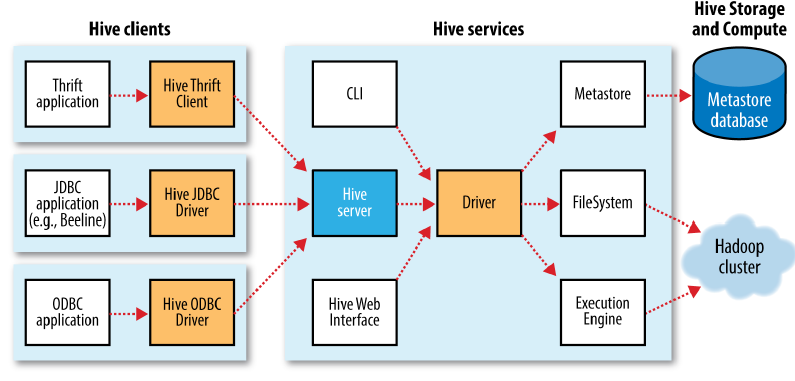
\includegraphics[width=\linewidth]{hiveSchema}
	\caption[Schéma de l'architecture de fonctionnement interne de Hive]{Schéma de l'architecture de fonctionnement interne de Hive \footnotemark}
\end{figure}

\footnotetext{Source: T. White, Hadoop: the definitive guide; [storage and analysis at Internet scale], 4. ed., Updated Beijing: O'Reilly, 2015. p.480}

Hive expose une liste de services et de fonctionnalité dans son architecture interne (Figure 2 - 8) :

\begin{itemize}
\item
Il propose 3 clients pour interagir avec Hive.  CLI (Hive Command line-interface) est le client Shell par défaut.  Beeline aussi une interface de line de commande ayant les mêmes fonctionnalités que le CLI avec la possibilité de connecté avec HiveServer 2 à travers un connecteur JDBC.  Le hwi (Hive Web Interface) est un simple client web au même titre que le CLI. 
\item
HiveServer2 est un service fournissant la possibilité de la connexion de multi utilisateurs (application) et d’authentification à Hive à travers Thrift, JDBC, et ODBC. 
\item
Hive Metastore est un service là pour le stockage des métadonnées concernant la structure des tables et des colonnes associées. Il rend à l’utilisateur une vision de base de données structurée. HCatalog est un API qui permet à d’autres applications d’avoir accès aux métadonnées de Hive Metastore. Hive Metastore peut être configuré de de 3 manière : 
	\begin{itemize}
	\item
	Embedded Metastore (Figure 2- 9) : ce mode utilise Derby comme base de données. La base Metastore et le service de Hive Metastore tournent dans le même processus d’exécution que Hive Server. Il ne peut qu’avoir qu’un utilisateur à la fois.
	\item
	Local Metastore (Figure 2 - 11) : Dans ce mode le service de Hive Metastore tourne dans le même processus d’exécution de HiveServer mais la base de Metastore tourne dans un processus différent et peut être dans un serveur distant.
	\item
	Remote Metastore (Figure 2 - 10) : dans ce mode, le service d’Hive Metastore s’exécute dans un processus séparé de Hive Server et de meme que la base Metastore. HiveServer2, Hcatalog et autre communique lui un API Thrift.
	\end{itemize}
\end{itemize}

En mode Local et Remote Metastore, le service Hive Metastore utilise un pilote JDBC pour communiquer à la base Metastore. 

\begin{figure}[H]
	\centering
	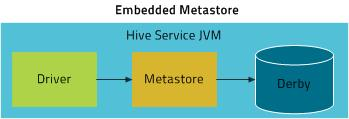
\includegraphics[width=6cm]{hiveEmbeddedMetaStore}
	\caption[Schéma processus Hive en mode Embedded Metastore]{Schéma de l'architecture de fonctionnement interne de Hive \footnotemark}
\end{figure}

\footnotetext{Source : \url{http://www.cloudera.com/documentation/cdh/5-1-x/CDH5-Installation-Guide/cdh5ig_hive_metastore\_configure.html}}


\begin{figure}[H]
	\centering
	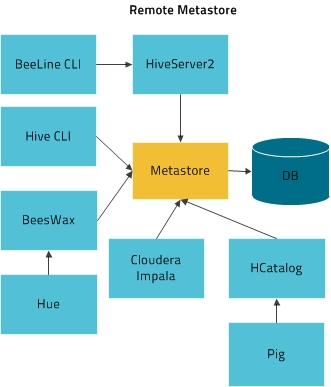
\includegraphics[width=6cm]{hiveRemoteMetaStore}
	\caption[Schéma processus Hive en mode Remote Metastore]{Schéma processus Hive en mode Remote Metastore}
\end{figure}

\begin{figure}[H]
	\centering
	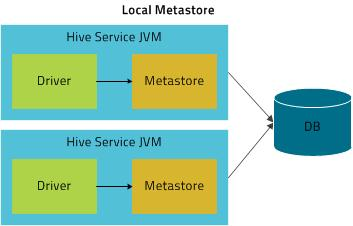
\includegraphics[width=6cm]{hiveLocalMetaStore}
	\caption[Schéma processus Hive en mode Local Metastore]{Schéma processus Hive en mode Local Metastore}
\end{figure}

\subsection{Installation de Hive 2.3.0 dans un cluster Hadoop}

Cette section montre comment installer Hive sur un cluster d’Hadoop existant (cluster configuré précédemment). Comme on peut voir sur le schéma suivant (figure x), Hive sera mis sur le nœud maitre (Master Node). La configuration sera en « Mode Remote » avec la base de données MySQL pour le stockage des métadonnées en provenance du service de Hive Metastore.

\begin{figure}[H]
	\centering
	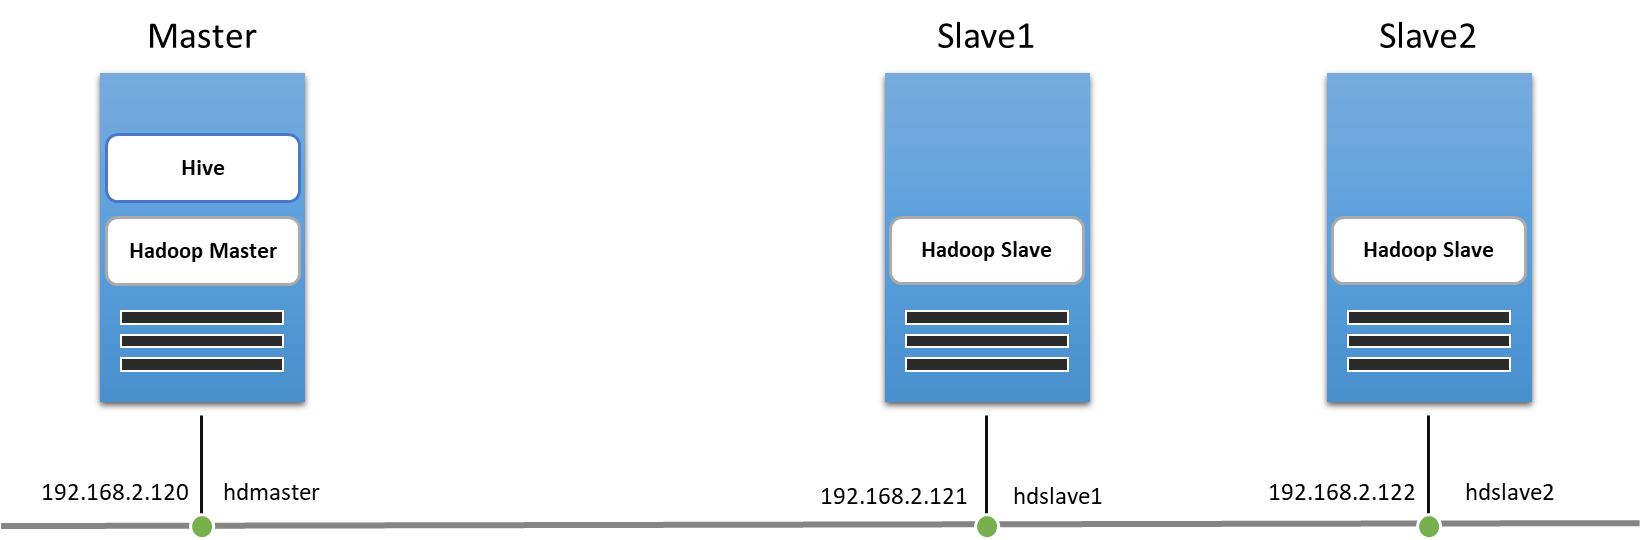
\includegraphics[width=\linewidth]{hiveCluster}
	\caption{Schéma de configuration de Hive sur le cluster d'Hadoop}
\end{figure}

\subsubsection{Prérequis}

Pour cette configuration de Hive, l’installation du cluster Hadoop doit être déjà mise en place, avec toutes les configurations nécessaires tel que Java 8, création de l’utilisateur, configuration de fichier /etc/hosts (voir section 2.5).

\subsubsection{Pré-configuration pour Hive}

Pour la configuration de Hive qui sera effectué, des mises en place sont nécessaires avant de passer à son installation.
Dans une première étape, s’effectuera l’installation, configuration de MySQL et mise en place de la base de données pour les données du service de Hive Metastore.
Dans un second temps, s’effectuera la création de répertoires d’utilisation de Hive dans HDFS.

\paragraph{Installation de MySQL pour Hive Metastore}\mbox{}\\


Lancer cette commande pour procéder à l’installation de MySQL

\begin{lstlisting}[language=bash, frame=single]
sudo apt-get install mysql-server
\end{lstlisting}

Lancer les services de mysql

\begin{lstlisting}[language=bash, frame=single]
sudo service mysql start
\end{lstlisting}

Installation du connecteur de MySQL.
Ce connecteur permettra à Hive Metastore service de se connecter à la base de données qui sera créée dans MySQL.
Hive fait usage de pilote JDBC pour communiquer avec MySQL.

\begin{lstlisting}[language=bash, frame=single]
sudo apt-get install libmysql-java
\end{lstlisting}

Création d’un lien symbolique dans le répertoire lib de Hive afin qu’il puise avoir une référence dans connecteur JDBC chez lui.

\begin{lstlisting}[language=bash, frame=single, breaklines=true, postbreak=\mbox{\textcolor{red}{$\hookrightarrow$}\space}]]
sudo ln -s /usr/share/java/mysql-connector-java.jar /usr/local/hive/lib/mysql-connector-java.jar
\end{lstlisting}

Renforcement de sécurité de MySQL avec l’utilitaire de sécurité

\begin{lstlisting}[language=bash, frame=single]
sudo /usr/bin/mysql_secure_installation
\end{lstlisting}

Faites comme suit :

\begin{lstlisting}[language=bash, frame=single]
...
Enter current password for root (enter for none):
OK, successfully used password, moving on...
...
Set root password? [Y/n] y
New password:
Re-enter new password:
Remove anonymous users? [Y/n] Y
...
Disallow root login remotely? [Y/n] N
...
Remove test database and access to it [Y/n] Y
...
Reload privilege tables now? [Y/n] Y
All done!
\end{lstlisting}

Changer le paramètre bind-address dans le fichier mysqld.cnf par son adresse IP du serveur pour avoir un accès distant à la base de données.

\begin{lstlisting}[language=bash, frame=single]
sudo nano /etc/mysql/mysql.conf.d/mysqld.cnf 
\end{lstlisting}

\begin{lstlisting}[language=bash, frame=single]
#find this line and change localhost to your server-ip
bind-address            = 192.168.2.120
\end{lstlisting}

Connecter en tant que root à MySQL

\begin{lstlisting}[language=bash, frame=single]
mysql -u root -p
enter password:
\end{lstlisting}

Dans l’invite de commande de MySQL, utiliser la commande suivante pour créer la base de données de Hive Metastore à partir du fichier hive-schema-2.3.0.mysql.sql qui permet de créer la base de données de MySQL pour la version 2.3.0 de Hive.
Ce script se trouve déjà à votre disposition dans les répertoires de Hive.

\begin{lstlisting}[language=SQL, frame=single, breaklines=true, postbreak=\mbox{\textcolor{red}{$\hookrightarrow$}\space}]
CREATE DATABASE metastore;
USE metastore;
SOURCE  /usr/local/hive-2.3.0/scripts/metastore/upgrade/mysql/hive-schema-2.3.0.mysql.sql
\end{lstlisting}

Toujours dans l’invite de commande de MySQL, passer les commandes suivantes pour la creation de l’utilisateur hive pour donner access à la base metastore au service de Hive. 

\begin{lstlisting}[language=SQL, frame=single, breaklines=true, postbreak=\mbox{\textcolor{red}{$\hookrightarrow$}\space}]
CREATE USER 'hive'@'hdmaster' IDENTIFIED BY 'hive!hive';
REVOKE ALL PRIVILEGES, GRANT OPTION FROM 'hive'@'hdmaster';
GRANT ALL PRIVILEGES ON metastore.* TO 'hive'@'hdmaster';

CREATE USER 'hive'@'%' IDENTIFIED BY 'hive!hive';
REVOKE ALL PRIVILEGES, GRANT OPTION FROM 'hive'@'%';
GRANT ALL PRIVILEGES ON metastore.* TO 'hive'@'%';

CREATE USER 'hive'@'192.168.2.120' IDENTIFIED BY 'hive!hive';
REVOKE ALL PRIVILEGES, GRANT OPTION FROM 'hive'@'192.168.2.120';
GRANT ALL PRIVILEGES ON metastore.* TO 'hive'@'192.168.2.120';
FLUSH PRIVILEGES;
quit;
\end{lstlisting}

Arrêter et redémarrer le démon de MySQL pour prendre en compte les modifications des fichiers de configuration.

\begin{lstlisting}[language=bash, frame=single]
sudo /etc/init.d/mysql stop
sudo /etc/init.d/mysql start
\end{lstlisting}

Verifier bien si l’utilisateur hive à la possibilité de se connecter à MySQL à l’hôte hdmaster 

\begin{lstlisting}[language=bash, frame=single]
mysql -h hdmaster -u hive -p
\end{lstlisting}

\paragraph{Creation des répertoires d’utilisation de Hive dans HDFS}

Créer dans HDFS  2 répertoires et assigner les droit lecture et écriture :  /tmp répertoire de données temporaire de Hive lors de l’exécution de tâches et /user/hive/warehouse répertoire pour la création des bases et tables. 

\begin{lstlisting}[language=bash, frame=single]
hdfs dfs -mkdir       /tmp
hdfs dfs -mkdir       /user/hive/warehouse

hdfs dfs -chmod g+w   /tmp
hdfs dfs -chmod g+w   /user/hive/warehouse
\end{lstlisting}

\paragraph{Installation de Hive}\mbox{}\\

On fera usage de la version 2.2.0 de Hive.
La version binaire d’Apache Hive peut être récupéré sur le site officiel (https://hive.apache.org/)
Allez dans le répertoire partager pour que Hive puisse être exécuté par un autre utilisateur.
Nous faisons le choix du répertoire /usr/local/ pour l’installation comme pour l’installation d’Hadoop.

\begin{lstlisting}[language=bash, frame=single]
cd /usr/local/ 
\end{lstlisting}

Allez sur le site offciel de hive dans téléchargement pour trouver le lien.

\begin{lstlisting}[language=bash, frame=single]
sudo wget http://apache.mirrors.ovh.net/ftp.apache.org/dist/hive/hive-2.3.0/apache-hive-2.3.0-bin.tar.gz
\end{lstlisting}

Désarchiver le fichier nouvellement téléchargé (ici apache-hive-2.3.0-bin.tar.gz) et renommer le répertoire obtenu en hive-2.3.0.

\begin{lstlisting}[language=bash, frame=single]
sudo tar -zxf apache-hive-2.3.0-bin.tar.gz
sudo mv apache-hive-2.3.0-bin hive-2.3.0
\end{lstlisting}

Donner l’utilisateur hdb la propriété sur répertoire

\begin{lstlisting}[language=bash, frame=single]
sudo chown hdb:hadoop -R /usr/local/hive-2.3.0
\end{lstlisting}

\paragraph{Mise en place des variables d’environnement d’Hive}

Se connecter en tant que hdb

\begin{lstlisting}[language=bash, frame=single]
sudo su hdb
\end{lstlisting}

Ajouter les variables d’environnement d’Hive dans le fichier profile de l’utilisateur hdb

\begin{lstlisting}[language=bash, frame=single]
nano /home/hdb/.bashrc
\end{lstlisting}

\begin{lstlisting}[language=bash, frame=single]
#Add to the end of this file 
# -- HIVE ENVIRONMENT VARIABLE START -- #
export HIVE_HOME=/usr/local/hive-2.3.0
export PATH=$PATH:$HIVE_HOME/bin
export CLASSPATH=$CLASSPATH:usr/local/hadoop-2.8.0/lib/*:.
export CLASSPATH=$CLASSPATH:/usr/local/hive-2.3.0/lib/*:.

# -- HIVE ENVIRONMENT VARIABLE END -- #
\end{lstlisting}

Rendre la modification du fichier profile active immédiatement
\begin{lstlisting}[language=bash, frame=single]
source /home/hdb/.bashrc
\end{lstlisting}

\paragraph{Configuration de Hive en mode « Remote Metastore » }\mbox{}\\

Référencer dans hive-config.sh le répertoire d’utilisation d’Hadoop

\begin{lstlisting}[language=bash, frame=single]
sudo nano /usr/local/hive-2.3.0/bin/hive-config.sh 
\end{lstlisting}

Chercher dans le fichier les lignes suivantes :
% REMOVE \$
\begin{lstlisting}[language=bash, frame=single]
# Allow alternate conf dir location.
HIVE_CONF_DIR="\${HIVE_CONF_DIR:-$HIVE_HOME/conf"
export HIVE_CONF_DIR=$HIVE_CONF_DIR
export HIVE_AUX_JARS_PATH=\$HIVE_AUX_JARS_PATH
\end{lstlisting}

Ajouter en dessous de ces lignes

\begin{lstlisting}[language=bash, frame=single]
export HADOOP_HOME=/usr/local/hadoop-2.8.0
\end{lstlisting}

Créer le fichier hive-site.xml à partir de la version par défaut fourni et l’éditer pour faire la configuration de Hive en mode Remonte Metastore.
Ce fichier permet d’indiquer à Hive les paramètre de connexion à la base et le nom des répertoires dans HDFS son utilisation.

\begin{lstlisting}[language=bash, frame=single]
cp hive-default.xml.template hive-site.xml
sudo gedit /usr/local/hive-2.3.0/conf/hive-site.xml 
\end{lstlisting}

Utilisez la commande ctrl + f pour accéder à l’option de rechercher (« find ») sur gedit afin de rechercher le nom (clef <name>) de votre propriété dont vous avez besoin et mettre les valeurs (clef <value>) nécessaires. 

\begin{lstlisting}[language=XML, frame=single, breaklines=true, postbreak=\mbox{\textcolor{red}{$\hookrightarrow$}\space}]
<property>
    <name>javax.jdo.option.ConnectionURL</name>
    <value>jdbc:mysql://hdmaster:3306/metastore</value>
    <description>
      JDBC connect string for a JDBC metastore.
      To use SSL to encrypt/authenticate the connection, provide database-specific SSL flag in the connection URL.
      For example, jdbc:postgresql://myhost/db?ssl=true for postgres database.
    </description>
</property>

<property>
    <name>javax.jdo.option.ConnectionDriverName</name>
    <value>com.mysql.jdbc.Driver</value>
    <description>Driver class name for a JDBC metastore</description>
</property>

<property>
    <name>javax.jdo.option.ConnectionUserName</name>
    <value>hive</value>
    <description>Username to use against metastore database</description>
</property>
<property>
    <name>javax.jdo.option.ConnectionPassword</name>
    <value>hive!hive</value>
    <description>password to use against metastore database</description>
</property>

<property>
    <name>hive.metastore.uris</name>
    <value>thrift://192.168.2.120:9083</value>
    <description>Thrift URI for the remote metastore. Used by metastore client to connect to remote metastore.</description>
  </property>

<property>
    <name>hive.metastore.warehouse.dir</name>
    <value>/user/hive/warehouse</value>
    <description>location of default database for the warehouse</description>
</property>

<property>
    <name>hive.exec.local.scratchdir</name>
    <value>/tmp/hive</value>
    <description>Local scratch space for Hive jobs</description>
</property>

<property>
    <name>hive.downloaded.resources.dir</name>
    <value>/tmp/hive/\${hive.session.id}_resources</value>
    <description>Temporary local directory for added resources in the remote file system.</description>
</property>

<property>
    <name>hive.scratch.dir.permission</name>
    <value>777</value>
    <description>The permission for the user specific scratch directories that get created.</description>
</property>
\end{lstlisting}

% remove the \$ on top!

\subsubsection{Démarrage des services de Hive}

Pour pouvoir se connecter, créer et manipuler des données sur Hive, il est necessaire de lancer ses services. Le service Metastore lancer et en exécution permet dès et déjà de pouvoir tirer usage du client CLI de Hive.  Le service de HiveServer2, d'un autre côté, doit être en exécution si nécessaire de connecter d’autres types d’application à Hive.  Car c’est ce service qui fait office de médium d’accès à Beeline et autres langages de programmation. Il faut aussi assurer que les démons Hadoop (HDFS et Yarn) sont bien démarrés.

Démarrer le service Metastore de Hive

\begin{lstlisting}[language=bash, frame=single]
hive   --service metastore
\end{lstlisting}

A cette étape-là, Le client de base de Hive, CLI permet déjà de faire des manipulations au niveau de la base de données de Hive.

Utilisation du client CLI :
\begin{lstlisting}[language=bash, frame=single]
hive 
\end{lstlisting}

Dans le client CLI hive, passer les commandes suivantes :

\begin{lstlisting}[language=bash, frame=single]
hive> show databases;
hive> use default;
hive> show tables;
\end{lstlisting}

« show databases » pour afficher la liste des base de données, « use default » pour indiquer l’utilisation de la base de données « default », base par défaut  de hive, « show tables » pour voir la liste des tables dans la base indiquée.

Démarrer le service HiveServer2 de Hive

\begin{lstlisting}[language=bash, frame=single]
hiveserver2
\end{lstlisting}

Les services HiveServer2 est nécessaire pour se connecter à Hive à travers le client Beeline et d’autres programme voulant s’y connecter

Une fois ce service lancé, les autres types clients incluant Beeline peuvent se connecter à la base de données de Hive.
Utilisation du client Beeline :

\begin{lstlisting}[language=bash, frame=single]
beeline
\end{lstlisting}

Connecter à Hive à travers Beeline

\begin{lstlisting}[language=bash, frame=single]
beeline> !connect jdbc:hive2://192.168.2.120:10000/  "" ""
\end{lstlisting}

\subsubsection{Exemple simple d’utilisation de Hive}

Dans cet exemple, montre la création d’une base « movielens » et la création d’une table « m\_rating » qui sera remplie à partir d’un fichier.
L’exemple utilise les données et fichiers en provenance de « Grouplens ».
voir lien permanant de « MovieLens 100K Dataset » pour plus d’information (http://grouplens.org/datasets/movielens/100k/). 

Se connecter à Hive à travers Beeline pour procéder à la creation de la Base de données « movielens ». Utiliser l’instruction qui suite :

\begin{lstlisting}[language=bash, frame=single]
beeline>CREATE DATABASE movielens;
\end{lstlisting}

Indiquer l’utilisation de la base movielens avec le mot clef USE :

\begin{lstlisting}[language=bash, frame=single]
beeline> USE movielens;
\end{lstlisting}

Utiliser cette instruction pour créer une tables nommée m\_rating dans la base nouvellement créée :

\begin{lstlisting}[language=SQL, frame=single]
CREATE TABLE m_rating (
u_id INT,
m_id INT,
rating INT,
timestmp STRING)
ROW FORMAT DELIMITED 
FIELDS TERMINATED BY '\t'
STORED AS TEXTFILE;
\end{lstlisting}

Télécharger le fichier zip de MovieLens en le plaçant dans le répertoire par défaut de l’utilisateur hdb et le désarchiver en étant hors de Beeline.  

\begin{lstlisting}[language=bash, frame=single, breaklines=true, postbreak=\mbox{\textcolor{red}{$\hookrightarrow$}\space}]]
sudo su hdb
cd ~
wget  http://files.grouplens.org/datasets/movielens/ml-100k.zip
unzip  ml-100k.zip
\end{lstlisting}

Retourner dans Beeline pour charger le fichier u.data et insérer les lignes dans la tables m\_rating en utilisant l’instruction suivante :

\begin{lstlisting}[language=bash, frame=single]
LOAD DATA LOCAL INPATH '/home/hdb/ml-100k/u.data'
OVERWRITE INTO TABLE m_rating;
\end{lstlisting}

Vérifier si les lignes ont bien été charger dans la table avec la requête suivante.

\begin{lstlisting}[language=bash, frame=single]
beeline> select * from m_rating limit 10;
\end{lstlisting}

Cette requête permet de calculer la moyenne des Indices « rating » pour chaque film représenté par son identifiant « m\_id » 

\begin{lstlisting}[language=bash, frame=single, breaklines=true, postbreak=\mbox{\textcolor{red}{$\hookrightarrow$}\space}]]
beeline> SELECT m_id, avg(rating) FROM m_rating GROUP BY m_id ;
\end{lstlisting}

Un aperçu du résultat partiel obtenu :

\begin{lstlisting}[language=bash, frame=single]
+-------+---------------------+--+
| m_id  |         _c1         |
+-------+---------------------+--+
| 1     | 3.8783185840707963  |
| 2     | 3.2061068702290076  |
| 3     | 3.033333333333333   |
| 4     | 3.550239234449761   |
| 5     | 3.302325581395349   |
| 6     | 3.576923076923077   |
| 7     | 3.798469387755102   |
| 8     | 3.9954337899543377  |
| 9     | 3.8963210702341136  |
| 10    | 3.831460674157303   |
| 11    | 3.847457627118644   |
| 12    | 4.385767790262173   |
| 13    | 3.4184782608695654  |
| 14    | 3.9672131147540983  |
| 15    | 3.7781569965870307  |
...
\end{lstlisting}

\section{Spark}

Apache Spark est un Framework écrit en Scala pour procéder à de l’analyse de données en utilisant des processus de traitement de données en mémoire dans un environnement distribué.

Spark et Hadoop forment un couple souvent utiliser par les entreprises pour le traitement et l’analyse de données stockées dans HDFS. La raison est d’une part Spark convient le mieux par sa capacité d’effectuer des traitements en temps réel (vitesse de traitement élevée), des analyses avancées et Hadoop en revanche, convient mieux le mieux pour le stockage de données allant de structurées au non-structurées et l’exécution de processus batch (temps différé) pour le traitement sur ces dernières.
Cette combinaison en couple permet de tirer avantage de la capacité de stockage d’Hadoop et la vitesse de traitement et d’analyse de Spark.    


\begin{figure}[h]
	\centering
	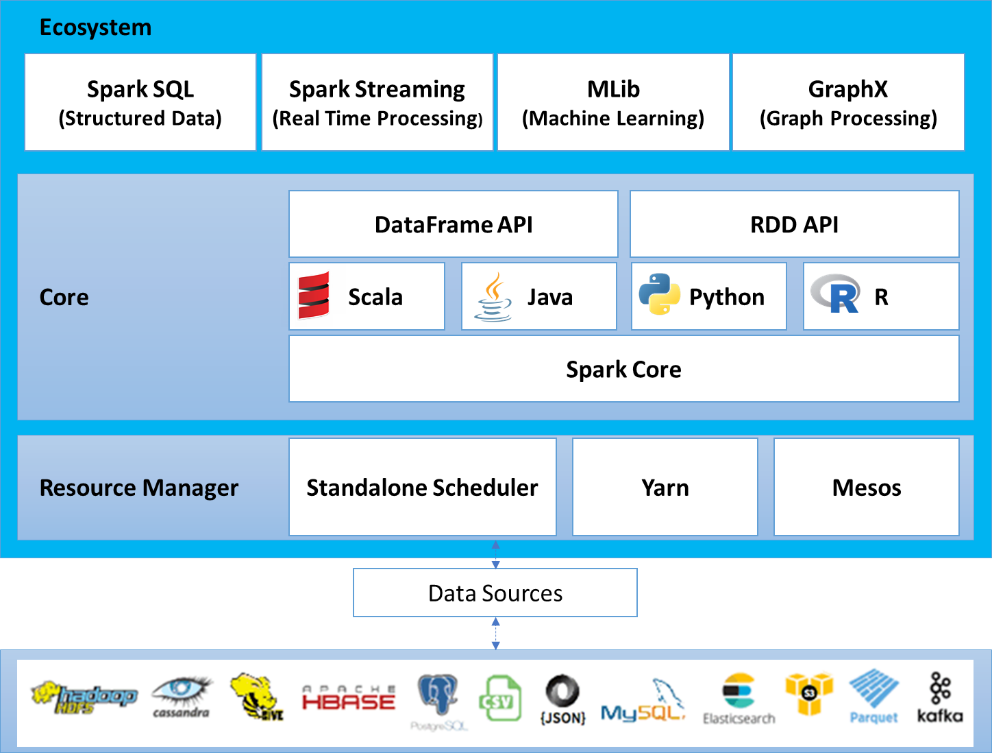
\includegraphics[width=10cm]{sparkSchema}
	\caption{Schéma des Composants de Spark}
\end{figure}

Apache Spark est un regroupement de composants (Figure 2 - 13) qui fonctionne autour du noyau de Spark (Spark Core).
Autour du noyau s’intègre des services, des APIs et des librairies de haut niveau.

Spark met à la disposition des programmeurs un ensemble de librairies et de différents langages pour réaliser une application capable d’être exécuté sur un cluster Spark et de produire des codes dans un langage qui convient le mieux au programmeur.
Parmi les librairies disponibles actuellement pour l’accomplissement d’application se trouvent MLib pour le Machine Learning, GraphX pour les traitements de données graphes en parallèles et SparkR pour travailler avec le langage R dans l’environnement cluster de Spark.
D’autres langages s’ajoutent à la liste comme Java, Scala, Python et SQL.

Spark offre deux (2) APIs, DataFrames et Resilient Distributed Datasets (RDDs). Les DataFrames (API non-typé) et les DataSets (API typé) fournissent une vision de fonctionnement pour l’utilisateur, son mode de fonctionnement réel dans Spark.
Pour un utilisateur, ils sont des tables représentées par des lignes et des colonnes distribuées en mémoire sur le cluster.
Pour Spark, ceux sont des tables immutables à évolution lente.
Spark gère le traitement de données structurées avec SQL ou à travers les Dataframes et les DataSets.
Les RDDs en revache, est l’abstraction de plus bas niveau de Spark représentant une collection d’éléments immutable et partitionnée utilisable en parallèle sur cluster.
Pour un utilisateur, chaque ligne représente un objet Java.
Ce qui lui donne un contrôle complet et une facilité dans la manipulation des données.
Un RDD étant l’abstraction de base, lors de la compilation du code ou se trouve des DataFrames ou des DataSets seront transformés chacun en RDD.

Spark SQL est un module pour travailler avec les données structurées.
Spark SQL est utilisé pour l’exécution des requête SQL ou à travers le DataFrame API utilisable dans les langage Java, Python, Scala et R.
SQL et DataFrames combinées fournit un moyen commun pour accéder à une variété de sources de données tel que Hive, Avro, Parquet, ORC, JSON, CSV, JDBC et ODBC.

Spark Streaming est un module dans spark pour la réalisation d’application de traitement de données en temps réel.
Streaming apporte la capacité de concevoir des applications interactives interactive d’analyse, de surveillance et de détection.
Il donne aussi la possibilité de réutiliser le même code de traitement batch, d’effectuer des jointures de données de diffusion (en acquisition temps réel) et des données Historiques ou d’exécuter des requêtes sur des données en mode diffusion (temps réel).

\begin{figure}[h]
	\centering
	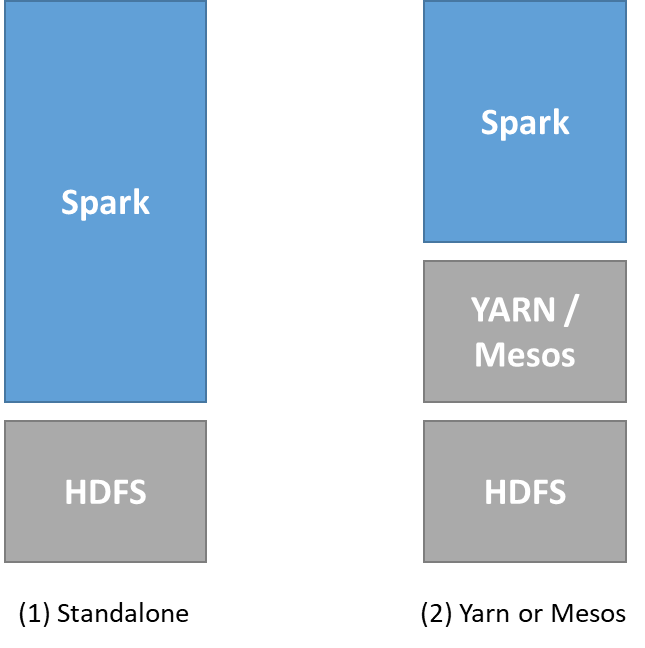
\includegraphics[width=10cm]{sparkConfig}
	\caption{Schéma des modes de configuration de Spark}
\end{figure}

Dans un cluster, Spark nécessite un gestionnaire de ressources (Resource Manager ou Cluster manager) pour l’optimisation, la surveillance (ou le contrôle d’activité) et l‘attribution d’exécution de taches sur le cluster.
Il supporte trois (3) types de gestionnaire de ressources dans une configuration en cluster (Figure 2 - 14).
Le mode “Standalone ou Native Cluster Manager” où le gestionnaire de ressource est celui de Spark.
Le mode « Yarn » utilisant le gestionnaire de ressource d’Hadoop, Yarn.
Le mode « Mesos » utilisant le gestionnaire de ressource indépendante Apache Mesos.
A noter que Spark est capable en un mode « Local » qui est un mode non-distribué.
Dans ce mode, tous ses processus sont dans un seul JVM sur une seule machine, idéal pour les tests et de débogage.

\begin{figure}[h]
	\centering
	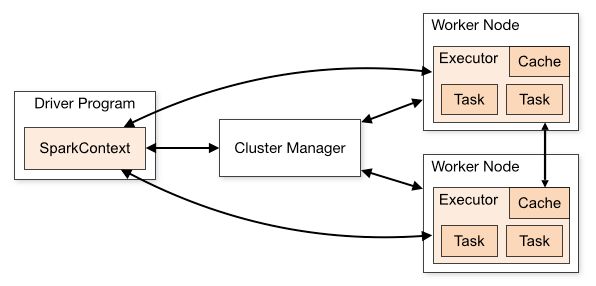
\includegraphics[width=\linewidth]{sparkArch}
	\caption[Schéma de l'architecture de fonctionnement de Spark en cluster]{Schéma de l'architecture de fonctionnement de Spark en cluster \footnotemark}
\end{figure}

\footnotetext{Source : \url{https://spark.apache.org/docs/latest/cluster-overview.html}}

Dans une architecture distribuée d’Apache Spark (Figure 2 - 15), une application Spark s’exécute en un ensemble de processus indépendante sur le cluster.
Un application Spark se compose d’une application principale nommé « Driver Program » et dans Driver program, le SparkContext qui est le coordinateur de ses propres processus s’exécutant sur le cluster.
Lors d’un lancement d’une application Spark, SparkContext contacte le gestionnaire de ressources du cluster, qui lui alloue des Executors dans des nœuds esclaves (Works Node).
Un Executor est un processus ayant pour fonctionne le traitement et le stockage de données pour l’application s’exécutant, à savoir le SparkContext garant de ce processus.
Mainteant que le SparkContext est en communication direct avec ses Executors, il peut à présent envoyer le code de l’application aux Executors et qui par la suite envoie les taches aux Executors pour être traitées.
Le code de l’application envoyé est soit un JAR ou un fichier Python qui est transmis à SparkContext.


\subsection{Installation de Apache Spark 2.2.0 un cluster}

Cette section montre comment installer Spark en cohabitation avec Hadoop dans un cluster existant (cluster configuré précédemment).
Comme on peut voir sur le schéma suivant (Figure 2 - 16), Spark Master sera mis sur le Master Node, le même que celui d’Hadoop Master et deux (2) Spark Slave sur les autres nœuds du cluster (Slave1 et Slave2).
Il s'agit d'utiliser Spark avec Yarn, le même gestionnaire de ressources utilisé par Hadoop.
Cela signifie que Spark et Hadoop partageront les mêmes ressources (RAM, CPU, disque). Le Yarn, en tant que gestionnaire de ressources de tous les deux, a la responsabilité de bien équilibrer l'allocation de ressources sur les nœuds esclaves (Slave Node).

\begin{figure}[h]
	\centering
	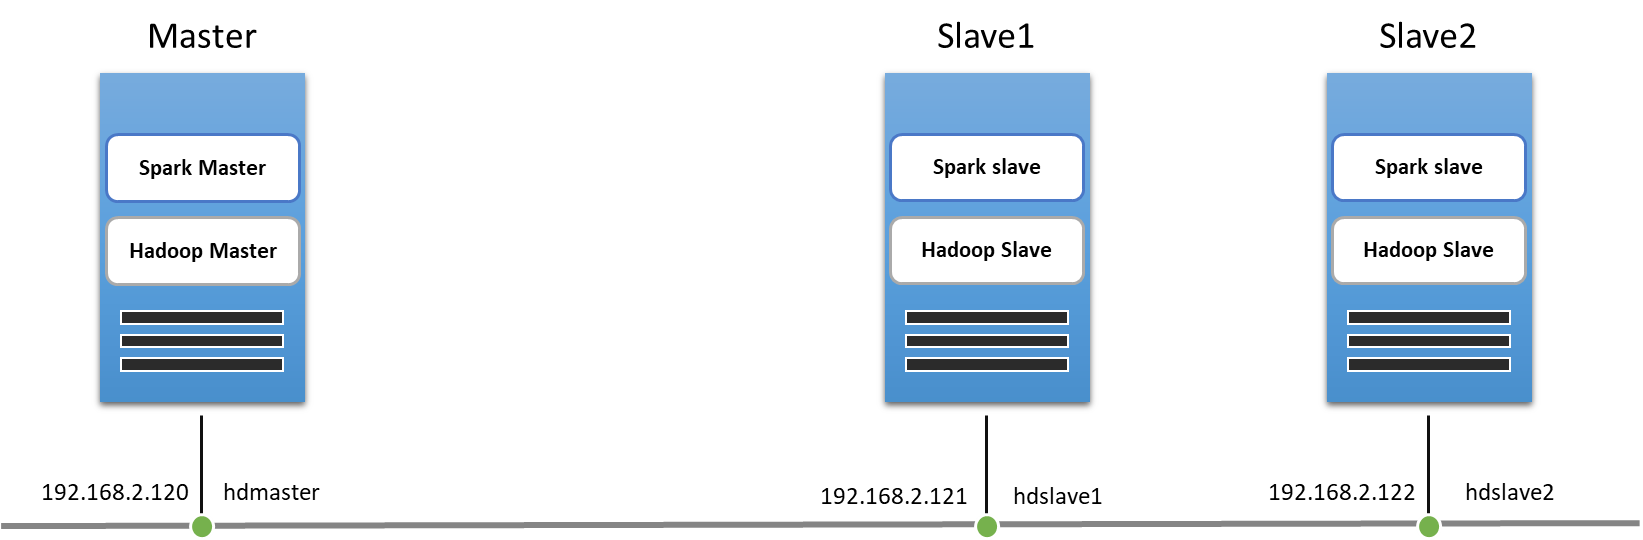
\includegraphics[width=\linewidth]{sparkCluster}
	\caption{Schéma de configuration de Spark sur le cluster d'Hadoop}
\end{figure}

\subsubsection{Prérequis}

Pour cette configuration de Spark en cluster, l’installation du cluster Hadoop doit être déjà mise en place, avec toutes les configurations nécessaires tel que Java 8, création de l’utilisateur hdb, installation de SSH serveur, génération de clef avec ssh-keygen pour l’utilisateur hdb sur toutes les machines du cluster, configuration de fichier /etc/hosts (voir section 2.5).
Spark est un Framework écrit en scala, il lui faut Scala pour fonctionner.
Ce qui fait que Spark a aussi besoin de Java pour son fonctionnement Car Scala est basé sur ce dernier.

\subsubsection{Installation de Scala}

La version de Spark 2.2.0 est compiler avec la version 2.11.0 de Scala,
Il est recommandé d’utiliser la même version de compilation.
Cette version de Scala est trouvable sur le site officiel (https://www.scala-lang.org/download/2.11.11.html).
Cette étape doit être réalisée sur toutes les machine du cluster.

Aller dans le répertoire /usr/local/ comme pour l’installation des autres précédemment

\begin{lstlisting}[language=bash, frame=single]
cd /usr/local
\end{lstlisting}

Téléchargement de Scala

\begin{lstlisting}[language=bash, frame=single, breaklines=true, postbreak=\mbox{\textcolor{red}{$\hookrightarrow$}\space}]
sudo wget https://downloads.lightbend.com/scala/2.11.11/scala-2.11.11.tgz
\end{lstlisting}

Désarchiver le fichier nouvellement téléchargé (ici scala-2.11.11.tgz)

\begin{lstlisting}[language=bash, frame=single]
sudo tar -zxf  scala-2.11.11.tgz
\end{lstlisting}

Vérifier si Scala fonctionne
Se connecter en tant que hdb

\begin{lstlisting}[language=bash, frame=single]
sudo su hdb
\end{lstlisting}

Lancer Scala en tapant la commande suivante :

\begin{lstlisting}[language=bash, frame=single]
scala
\end{lstlisting}

Tapez cette instruction pour mettre fin à l'exécution de scala

\begin{lstlisting}[language=bash, frame=single]
:quit
\end{lstlisting}

\subsubsection{Installation de Spark}

La version binaire d’Apache Spark peut être récupéré sur le site officiel (https://spark.apache.org/).

Allez dans un répertoire partager pour que Spark puisse être exécuté par un autre utilisateur.
Nous faisons le choix du répertoire /usr/local/ comme pour l’installation des autres précédemment.
Cette étape doit être réalisée que sur le nœud « Master ».

\begin{lstlisting}[language=bash, frame=single]
cd /usr/local
\end{lstlisting}

Téléchargement de Spark

\begin{lstlisting}[language=bash, frame=single, breaklines=true, postbreak=\mbox{\textcolor{red}{$\hookrightarrow$}\space}]
sudo wget http://mirrors.standaloneinstaller.com/apache/spark/spark-2.2.0/spark-2.2.0-bin-hadoop2.7.tgz
\end{lstlisting}

Désarchiver le fichier nouvellement téléchargé (ici spark-2.2.0-bin-hadoop2.7.tgz) et renommer le répertoire obtenu en spark-2.2.0.

\begin{lstlisting}[language=bash, frame=single]
sudo tar xzf spark-2.2.0-bin-hadoop2.7.tgz 
sudo mv spark-2.2.0-bin-hadoop2.7  spark-2.2.0
\end{lstlisting}

Donner l’utilisateur hdb la propriété sur le répertoire

\begin{lstlisting}[language=bash, frame=single]
sudo chown hdb:hadoop spark-2.2.0
\end{lstlisting}

Aller dans le répertoire /conf/ de spark, copier le fichier modèle pour créer le fichier d’environnement Spark (spark-env.sh) et Ajouter le fichier les variables qui suit.

\begin{lstlisting}[language=bash, frame=single]
cd /usr/local/spark-2.2.0/conf/

sudo cp spark-env.sh.template spark-env.sh

sudo nano spark-env.sh
\end{lstlisting}

\begin{lstlisting}[language=bash, frame=single]
export JAVA_HOME=/usr/lib/jvm/java-8-oracle

export SPARK_WORKER_CORES=2
\end{lstlisting}

Toujours dans le répertoire /conf/, éditer le fichier « slaves » les alias correspondant aux adresse IP de tous les nœuds esclaves du cluster afin d’indiquer à Spark, les machines agissant comme esclave.
Ici, les esclaves sont « hdslave1 » et « hdslave2 »

\begin{lstlisting}[language=bash, frame=single]
sudo nano /usr/local/spark-2.2.0/conf/slaves
\end{lstlisting}

\begin{lstlisting}[language=bash, frame=single]
hdslave1
hdslave2
\end{lstlisting}

\paragraph{Mise en place des variables d’environnement de Spark}\mbox{}\\

Pour le fonctionnement, une mise en place de variables d’environnement dans le profil de l’utilisateur responsable de l’exécution de Spark doit être effectuées.
Cette étape devra être réalisée sur toutes les machine du cluster.

Se connecter en tant que hdb

\begin{lstlisting}[language=bash, frame=single]
sudo su hdb
\end{lstlisting}

Ajouter les variables d’environnement de Spark dans le fichier profile de l’utilisateur hdb

\begin{lstlisting}[language=bash, frame=single]
nano /home/hdb/.bashrc
\end{lstlisting}

\begin{lstlisting}[language=bash, frame=single]
# -- Spark ENVIRONMENT VARIABLE START -- #
export SPARK_HOME=/usr/local/spark-2.2.0
export PATH=$PATH:$SPARK_HOME/bin

export SCALA_HOME=/usr/local/scala-2.11.11
export PATH=$PATH:$SCALA_HOME/bin
# -- Spark ENVIRONMENT VARIABLE END -- #
\end{lstlisting}

Rendre la modification du fichier profile active immédiatement

\begin{lstlisting}[language=bash, frame=single]
source /home/hdb/.bashrc
\end{lstlisting}

Tester pour voir si Spark-Shell, la line de commande de spark fonctionne normalement avec la line suivante :

\begin{lstlisting}[language=bash, frame=single]
spark-shell
\end{lstlisting}

Tapez cette instruction pour mettre fin à l'exécution de spark-shell

\begin{lstlisting}[language=bash, frame=single]
:quit
\end{lstlisting}

\paragraph{Creation des répertoires d’utilisation de spark dans HDFS}\mbox{}\\

Créer dans HDFS le répertoire /user/spark/ et assigner les droit lecture et écriture pour l’exécution des tâches de spark. 

\begin{lstlisting}[language=bash, frame=single]
hdfs dfs -mkdir       /user/spark/
hdfs dfs -chmod g+w   /user/spark/
\end{lstlisting}

\subsubsection{Configuration installation et configuration de Spark sur les nœuds esclaves}\mbox{}\\

Pour la configuration les nœuds esclaves, elle se fera en dans partie.
Une partie, sur la machine Master qui consiste à récupérer la configuration initiale du nœud Master et de le copier sur les nœuds esclaves à savoir « hdslave1 » et « hdslave2 ».
La seconde sera effectuée sur les nœuds esclave. Cette seconde partie consiste à déployer le répertoire copié dans son environnement naturel et donner droit à l’utilisateur hdb sur ce dernier. 

\paragraph{Etape 1 à effectuer depuis le nœud Master}\mbox{}\\

Archiver le répertoire Spark avec tar :  

\begin{lstlisting}[language=bash, frame=single]
sudo tar czf spark-2.2.0.tar.gz spark-2.2.0
\end{lstlisting}

Copier par SSH le fichier archive de Spark sur tous les nœuds esclaves avec l’utilisateur hdb à partir des commandes qui suit :

\begin{lstlisting}[language=bash, frame=single]
sudo scp spark-2.2.0.tar.gz hdb@hdslave1:~
sudo scp spark-2.2.0.tar.gz hdb@hdslave2:~
\end{lstlisting}

\paragraph{Etape 2 à effectuer depuis les nœuds esclaves}\mbox{}\\

Etant sur chaque machine esclave, aller dans le répertoire /usr/local/ , désarchiver le fichier  spark-2.2.0.tar.gz qui se trouve dans /home/hdb/ et copier le répertoire (spark-2.2.0) nouvellement crée dans /usr/local/ en utilisant les commande suivantes :

\begin{lstlisting}[language=bash, frame=single]
cd /usr/local/
sudo tar xzf /home/hdb/spark-2.2.0.tar.gz 
sudo cp /home/hdb/spark-2.2.0.tar.gz spark-2.2.0
\end{lstlisting}

Donner l’utilisateur hdb la propriété sur le répertoire de Spark

\begin{lstlisting}[language=bash, frame=single]
sudo chown hdb:hadoop spark-2.2.0
\end{lstlisting}

\subsubsection{Démarrage des services des démons de Spark sur le cluster}

Arriver dans cette étape, on peut maintenant démarrer les démons de Spark sur les machines du cluster. De même que Hadoop, Spark peut mettre en route tous les démons Master et Workers à partir du nœud Master.

Lancer cette commande sur le noeud maître en tant que l’utilisateur hdb
%remove the \$
\begin{lstlisting}[language=bash, frame=single]
\$SPARK_HOME/sbin/start-all.sh 
\end{lstlisting}

Verifier sur le nœud maitre avec cette commande, si tous les démons sont en exécution. Le démon du maitre de Spark est « Master »

\begin{lstlisting}[language=bash, frame=single]
jps
\end{lstlisting}

\begin{lstlisting}[language=bash, frame=single]
20226 ResourceManager
19811 NameNode
11509 Jps
20038 SecondaryNameNode
11435 Master
\end{lstlisting}

Verifier sur les nœuds esclaves avec cette commande, si tous les démons sont en exécution. Le démon du nœud esclaves de Spark est « Worker »

\begin{lstlisting}[language=bash, frame=single]
jps
\end{lstlisting}

\begin{lstlisting}[language=bash, frame=single]
8561 Jps
8249 NodeManager
7753 DataNode
7964 Worker
\end{lstlisting}

Pour l’arrêter les démons de Spark, lancer le fichier \$SPARK\_HOME/sbin/stop-all.sh en étant l’utilisateur propriétaire de Spark.
Dans notre cas, l’utilisateur est hdb. 

\subsubsection{Exemple simple d’exécution d’application sur spark-shell avec Yarn}

Dans cette section, on verra à partir d’un exemple de MapReduce de compter de mot en Scala, comment exécuter et traiter des données à partir du Shell de Spark.
Dans cet exemple, le Shell de Spark sera connecté en tant de client de du gestionnaire de ressources de Hadoop Yarn.
Dans l’exemple, l’usage des fichiers test01 et test02 dans le répertoire /user/hdb/input\_ex dans HDFS crées précédemment.

Passer cette commande pour lancer le Spark-Shell en tant que client de yarn

\begin{lstlisting}[language=bash, frame=single, breaklines=true, postbreak=\mbox{\textcolor{red}{$\hookrightarrow$}\space}]]
\$SPARK_HOME/bin/spark-shell --master yarn --deploy-mode client
\end{lstlisting}

Après avoir exécuter spark-shell en tant que client yarn, exécuter le code compteur de mot dans l’invite Scala de Spark.
Le programme MapReduce en parametre en entrée (input) le répertoire (/user/hdb/input\_ex) dans HDFS où se trouve les fichiers test01 et test02 et en sortie (output) le répertoire (/user/hdb/output\_ex\_spark) pour le dépôt des résultats obtenus.
A noter que les liens de connexion vers HDFS est hdfs://hdmaster:9000, avec hdmaster, l’alias du nœud maitre et le port 9000 pour de connexion au service d’HDFS.

\begin{lstlisting}[language=bash, frame=single, breaklines=true, postbreak=\mbox{\textcolor{red}{$\hookrightarrow$}\space}]]
val textFile = sc.textFile("hdfs://hdmaster:9000/user/hdb/input_ex")
val text = textFile.flatMap(line => line.split(" "))
val map = text.map(word => (word, 1))
val reduce = map.reduceByKey(_ + _)
reduce.saveAsTextFile("hdfs://hdmaster:9000/user/hdb/output_ex_spark")
\end{lstlisting}

Les résultats sont dans le fichiers part-00000 à part-xxxx.
Selon le volume d’information à stocker, il peut les séparer en plusieurs parties des numérotations continues avec le préfixe « part- ».

Afficher les résultats obtenus :

\begin{lstlisting}[language=bash, frame=single]
hadoop fs -cat  /user/hdb/output_ex_spark/part-*
\end{lstlisting}

\begin{lstlisting}[language=bash, frame=single]
(Bye,1)
(Welcome,1)
(Hello,2)
(Yarn,2)
(HDFS,1)
(Hadoop,1)
\end{lstlisting}

\section{Références du Chapitre 2}

[1]T. White, Hadoop: the definitive guide ; [storage and analysis at Internet scale], 4. ed., Updated. Beijing: O'Reilly, 2015.

[2] Apache Hadoop official Documents [En Ligne] Disponible : https://wiki.apache.org/hadoop

[1]Manish A. Kukreja, « Apache Hive: Enterprise SQL on Big Data frameworks ». Unpublished, 2016.

[1]A. Thusoo et al., « Hive - a petabyte scale data warehouse using Hadoop », 2010, p. 996‑1005.

[1]A. Thusoo et al., « Hive: a warehousing solution over a map-reduce framework », Proceedings of the VLDB Endowment, vol. 2, no 2, p. 1626‑1629, août 2009.

[1]E. Capriolo, D. Wampler, et J. Rutherglen, Programming Hive: [data warehouse and query language for Hadoop], 1. ed. Beijing: O'Reilly, 2012.

[1]S. Ryza, U. Laserson, S. Owen, et J. Wills, Advanced analytics with Spark, First edition. Beijing ; Sebastopol, CA: O'Reilly, 2015.

[1]B. Chambers et M. Zaharia, Spark,  the definitive guide: big data processing made simple. 2017.

[1]J. Dean et S. Ghemawat, « MapReduce: simplified data processing on large clusters », Communications of the ACM, vol. 51, no 1, p. 107‑113, janv. 2008.

\end{document}
